\documentclass[10pt,a4paper]{article}
\usepackage[utf8]{inputenc}
\usepackage[T1]{fontenc}
\usepackage{lmodern}
\usepackage[hmargin=0.8in,vmargin=0.75in]{geometry}
\usepackage{amsmath,amssymb,amsthm}
\usepackage{booktabs}
\usepackage{graphicx}
\usepackage{microtype}
\usepackage[numbers,sort&compress]{natbib}
\usepackage{xcolor}
\usepackage[colorlinks=true,linkcolor=blue!50!black,citecolor=blue!50!black,urlcolor=blue!50!black]{hyperref}
\usepackage{enumitem}
\usepackage{array}
\newcolumntype{L}[1]{>{\raggedright\arraybackslash}p{#1}}
\usepackage{caption}
\usepackage[section]{placeins}
\setcounter{topnumber}{3}\setcounter{totalnumber}{4}
\renewcommand{\topfraction}{0.95}\renewcommand{\bottomfraction}{0.7}
\renewcommand{\textfraction}{0.05}\renewcommand{\floatpagefraction}{0.7}
\captionsetup{font=small,labelfont=bf,skip=5pt}
\setlength{\bibsep}{0.5pt plus 0.5pt}
\setlength{\textfloatsep}{9pt plus 2pt minus 2pt}\setlength{\floatsep}{8pt plus 2pt minus 2pt}\setlength{\intextsep}{8pt plus 2pt minus 2pt}

\IfFileExists{numbers.tex}{% generated by experiments/make_numbers.py -- do not edit
\newcommand{\MetaSeed}{20260930}
\newcommand{\MetaR}{20\,000}
\newcommand{\MetaSeconds}{17}
\newcommand{\MetaPython}{3.11.15}
\newcommand{\MetaNumpy}{2.4.6}
\newcommand{\MetaScipy}{1.17.1}
\newcommand{\MetaMpl}{3.11.2}
\newcommand{\Cd}{5}
\newcommand{\CS}{30}
\newcommand{\Cns}{60}
\newcommand{\Cn}{60}
\newcommand{\Cm}{12}
\newcommand{\Cne}{48}
\newcommand{\CsnrDep}{1}
\newcommand{\CnConfigs}{345}
\newcommand{\CnOps}{3}
\newcommand{\CsnrGrid}{0, 0.25, 0.5, 1, 2, 4, 8, 16}
\newcommand{\CdepGrid}{0, 2, 4, 6, 8, 12, 16}
\newcommand{\CmGrid}{3, 6, 12, 24}
\newcommand{\CalphaGrid}{0.5, 0.2, 0.1, 0.05, 0.01}
\newcommand{\CuseThr}{5.0\%}
\newcommand{\SplitCost}{25.0\%}
\newcommand{\RefRiskE}{0.1042}
\newcommand{\RefRiskN}{0.0833}
\newcommand{\KappaHalf}{0.1700}
\newcommand{\PhizHalf}{0.3989}
\newcommand{\RatioHalf}{0.43}
\newcommand{\KappaTwenty}{0.0451}
\newcommand{\PhizTwenty}{0.2800}
\newcommand{\RatioTwenty}{0.16}
\newcommand{\KappaTen}{0.0188}
\newcommand{\PhizTen}{0.1755}
\newcommand{\RatioTen}{0.11}
\newcommand{\KappaFive}{0.0082}
\newcommand{\PhizFive}{0.1031}
\newcommand{\RatioFive}{0.08}
\newcommand{\KappaOne}{0.0013}
\newcommand{\PhizOne}{0.0267}
\newcommand{\RatioOne}{0.05}
\newcommand{\SafeAll}{yes}
\newcommand{\SafeHarmAll}{yes}
\newcommand{\MaxExcessOverPhi}{0.42}
\newcommand{\MaxRegretOverBound}{0.42}
\newcommand{\MaxIdentityZ}{2.96}
\newcommand{\NIdentityCLT}{273}
\newcommand{\NIdentityPoisson}{72}
\newcommand{\NIdentityFail}{2}
\newcommand{\UsefulRevHalf}{0, 0.25, 0.5, 1, 2}
\newcommand{\UsefulRefitHalf}{0, 0.25, 0.5, 1, 2, 4}
\newcommand{\HarmMaxHalf}{25.3\%}
\newcommand{\AccHarmMaxHalf}{50.0\%}
\newcommand{\UsefulRevTwenty}{0, 0.25, 0.5}
\newcommand{\UsefulRefitTwenty}{0, 0.25, 0.5, 1, 2}
\newcommand{\HarmMaxTwenty}{7.7\%}
\newcommand{\AccHarmMaxTwenty}{18.2\%}
\newcommand{\UsefulRevTen}{0}
\newcommand{\UsefulRefitTen}{0, 0.25, 0.5, 1}
\newcommand{\HarmMaxTen}{3.4\%}
\newcommand{\AccHarmMaxTen}{8.4\%}
\newcommand{\UsefulRevFive}{none}
\newcommand{\UsefulRefitFive}{0, 0.25}
\newcommand{\HarmMaxFive}{1.5\%}
\newcommand{\AccHarmMaxFive}{4.3\%}
\newcommand{\UsefulRevOne}{none}
\newcommand{\UsefulRefitOne}{none}
\newcommand{\HarmMaxOne}{0.2\%}
\newcommand{\AccHarmMaxOne}{1.0\%}
\newcommand{\UsefulAlways}{0, 0.25, 0.5, 1, 2, 4, 8}
\newcommand{\UsefulSure}{0, 0.25, 0.5, 1, 2, 4, 8}
\newcommand{\HarmfulAlwaysDep}{4, 6, 8, 12, 16}
\newcommand{\HarmfulSureDep}{4, 6, 8}
\newcommand{\HarmfulRefitTenDep}{4, 6, 8, 12, 16}
\newcommand{\HarmfulRevTenDep}{0, 2, 4, 6, 8, 12, 16}
\newcommand{\WorstDep}{16}
\newcommand{\WorstAlways}{1.4383}
\newcommand{\WorstRatioAlways}{13.8}
\newcommand{\WorstRe}{0.1042}
\newcommand{\WorstRn}{0.0835}
\newcommand{\WorstRevHalf}{0.1454}
\newcommand{\WorstExcessHalf}{0.0412}
\newcommand{\WorstBoundPhiHalf}{0.2738}
\newcommand{\WorstBoundAlphaHalf}{0.6670}
\newcommand{\WorstRevTwenty}{0.1098}
\newcommand{\WorstExcessTwenty}{0.0055}
\newcommand{\WorstBoundPhiTwenty}{0.1921}
\newcommand{\WorstBoundAlphaTwenty}{0.2668}
\newcommand{\WorstRevTen}{0.1054}
\newcommand{\WorstExcessTen}{0.0012}
\newcommand{\WorstBoundPhiTen}{0.1204}
\newcommand{\WorstBoundAlphaTen}{0.1334}
\newcommand{\WorstRevFive}{0.1046}
\newcommand{\WorstExcessFive}{0.0004}
\newcommand{\WorstBoundPhiFive}{0.0708}
\newcommand{\WorstBoundAlphaFive}{0.0667}
\newcommand{\WorstRevOne}{0.1042}
\newcommand{\WorstExcessOne}{0.0000}
\newcommand{\WorstBoundPhiOne}{0.0183}
\newcommand{\WorstBoundAlphaOne}{0.0133}
\newcommand{\SZeroRn}{0.0833}
\newcommand{\SZeroRe}{0.1044}
\newcommand{\SZeroAlwaysGain}{+96.4\%}
\newcommand{\SZeroAlwaysHarm}{0.1\%}
\newcommand{\SZeroAlwaysEHarm}{0.1\%}
\newcommand{\SZeroRevHalfGain}{+64.6\%}
\newcommand{\SZeroRevHalfGainE}{+71.7\%}
\newcommand{\SZeroRevHalfHarm}{0.0\%}
\newcommand{\SZeroRevHalfAcc}{70.1\%}
\newcommand{\SZeroRevTwentyGain}{+26.7\%}
\newcommand{\SZeroRevTwentyGainE}{+41.6\%}
\newcommand{\SZeroRevTwentyHarm}{0.0\%}
\newcommand{\SZeroRevTwentyAcc}{38.3\%}
\newcommand{\SZeroRevTenGain}{+7.6\%}
\newcommand{\SZeroRevTenGainE}{+26.3\%}
\newcommand{\SZeroRevTenHarm}{0.0\%}
\newcommand{\SZeroRevTenAcc}{23.4\%}
\newcommand{\SZeroRevFiveGain}{-5.1\%}
\newcommand{\SZeroRevFiveGainE}{+16.2\%}
\newcommand{\SZeroRevFiveHarm}{0.0\%}
\newcommand{\SZeroRevFiveAcc}{14.0\%}
\newcommand{\SZeroRevOneGain}{-19.7\%}
\newcommand{\SZeroRevOneGainE}{+4.6\%}
\newcommand{\SZeroRevOneHarm}{0.0\%}
\newcommand{\SZeroRevOneAcc}{3.8\%}
\newcommand{\SZeroRefitTenGain}{+15.7\%}
\newcommand{\SZeroSureGain}{+78.8\%}
\newcommand{\SZeroPoolAlways}{0.0028}
\newcommand{\SZeroPoolRevTen}{0.0776}
\newcommand{\SOneRn}{0.0841}
\newcommand{\SOneRe}{0.1048}
\newcommand{\SOneAlwaysGain}{+42.3\%}
\newcommand{\SOneAlwaysHarm}{20.2\%}
\newcommand{\SOneAlwaysEHarm}{17.7\%}
\newcommand{\SOneRevHalfGain}{+21.5\%}
\newcommand{\SOneRevHalfGainE}{+37.1\%}
\newcommand{\SOneRevHalfHarm}{7.5\%}
\newcommand{\SOneRevHalfAcc}{63.0\%}
\newcommand{\SOneRevTwentyGain}{+3.0\%}
\newcommand{\SOneRevTwentyGainE}{+22.2\%}
\newcommand{\SOneRevTwentyHarm}{2.7\%}
\newcommand{\SOneRevTwentyAcc}{32.6\%}
\newcommand{\SOneRevTenGain}{-6.6\%}
\newcommand{\SOneRevTenGainE}{+14.5\%}
\newcommand{\SOneRevTenHarm}{1.3\%}
\newcommand{\SOneRevTenAcc}{19.6\%}
\newcommand{\SOneRevFiveGain}{-13.5\%}
\newcommand{\SOneRevFiveGainE}{+9.0\%}
\newcommand{\SOneRevFiveHarm}{0.6\%}
\newcommand{\SOneRevFiveAcc}{11.3\%}
\newcommand{\SOneRevOneGain}{-20.8\%}
\newcommand{\SOneRevOneGainE}{+3.1\%}
\newcommand{\SOneRevOneHarm}{0.1\%}
\newcommand{\SOneRevOneAcc}{3.4\%}
\newcommand{\SOneRefitTenGain}{+6.1\%}
\newcommand{\SOneSureGain}{+33.2\%}
\newcommand{\SOnePoolAlways}{0.1097}
\newcommand{\SOnePoolRevTen}{0.0999}
\newcommand{\SFourRn}{0.0833}
\newcommand{\SFourRe}{0.1052}
\newcommand{\SFourAlwaysGain}{+16.1\%}
\newcommand{\SFourAlwaysHarm}{33.0\%}
\newcommand{\SFourAlwaysEHarm}{30.7\%}
\newcommand{\SFourRevHalfGain}{-4.1\%}
\newcommand{\SFourRevHalfGainE}{+17.5\%}
\newcommand{\SFourRevHalfHarm}{11.9\%}
\newcommand{\SFourRevHalfAcc}{58.7\%}
\newcommand{\SFourRevTwentyGain}{-12.2\%}
\newcommand{\SFourRevTwentyGainE}{+11.1\%}
\newcommand{\SFourRevTwentyHarm}{4.1\%}
\newcommand{\SFourRevTwentyAcc}{29.2\%}
\newcommand{\SFourRevTenGain}{-16.7\%}
\newcommand{\SFourRevTenGainE}{+7.5\%}
\newcommand{\SFourRevTenHarm}{1.8\%}
\newcommand{\SFourRevTenAcc}{17.3\%}
\newcommand{\SFourRevFiveGain}{-20.1\%}
\newcommand{\SFourRevFiveGainE}{+4.8\%}
\newcommand{\SFourRevFiveHarm}{0.8\%}
\newcommand{\SFourRevFiveAcc}{10.2\%}
\newcommand{\SFourRevOneGain}{-23.9\%}
\newcommand{\SFourRevOneGainE}{+1.8\%}
\newcommand{\SFourRevOneHarm}{0.1\%}
\newcommand{\SFourRevOneAcc}{3.0\%}
\newcommand{\SFourRefitTenGain}{+2.5\%}
\newcommand{\SFourSureGain}{+12.7\%}
\newcommand{\SFourPoolAlways}{0.4291}
\newcommand{\SFourPoolRevTen}{0.1087}
\newcommand{\SSixteenRn}{0.0833}
\newcommand{\SSixteenRe}{0.1044}
\newcommand{\SSixteenAlwaysGain}{+4.4\%}
\newcommand{\SSixteenAlwaysHarm}{41.4\%}
\newcommand{\SSixteenAlwaysEHarm}{40.6\%}
\newcommand{\SSixteenRevHalfGain}{-17.2\%}
\newcommand{\SSixteenRevHalfGainE}{+6.5\%}
\newcommand{\SSixteenRevHalfHarm}{15.4\%}
\newcommand{\SSixteenRevHalfAcc}{54.6\%}
\newcommand{\SSixteenRevTwentyGain}{-19.8\%}
\newcommand{\SSixteenRevTwentyGainE}{+4.4\%}
\newcommand{\SSixteenRevTwentyHarm}{5.2\%}
\newcommand{\SSixteenRevTwentyAcc}{25.8\%}
\newcommand{\SSixteenRevTenGain}{-21.8\%}
\newcommand{\SSixteenRevTenGainE}{+2.9\%}
\newcommand{\SSixteenRevTenHarm}{2.4\%}
\newcommand{\SSixteenRevTenAcc}{14.6\%}
\newcommand{\SSixteenRevFiveGain}{-22.9\%}
\newcommand{\SSixteenRevFiveGainE}{+1.9\%}
\newcommand{\SSixteenRevFiveHarm}{1.1\%}
\newcommand{\SSixteenRevFiveAcc}{8.6\%}
\newcommand{\SSixteenRevOneGain}{-24.5\%}
\newcommand{\SSixteenRevOneGainE}{+0.7\%}
\newcommand{\SSixteenRevOneHarm}{0.1\%}
\newcommand{\SSixteenRevOneAcc}{2.3\%}
\newcommand{\SSixteenRefitTenGain}{+0.6\%}
\newcommand{\SSixteenSureGain}{+3.4\%}
\newcommand{\SSixteenPoolAlways}{1.7324}
\newcommand{\SSixteenPoolRevTen}{0.1064}
\newcommand{\DZeroRn}{0.0837}
\newcommand{\DZeroRe}{0.1044}
\newcommand{\DZeroAlwaysRatio}{0.58}
\newcommand{\DZeroAlwaysEHarm}{17.2\%}
\newcommand{\DZeroRevHalfRatio}{0.78}
\newcommand{\DZeroRevHalfHarm}{7.2\%}
\newcommand{\DZeroRevHalfExcess}{-0.0388}
\newcommand{\DZeroRevHalfBoundPhi}{0.0513}
\newcommand{\DZeroRevHalfBoundAlpha}{0.0019}
\newcommand{\DZeroRevHalfBoundTight}{0.0014}
\newcommand{\DZeroRevTwentyRatio}{0.97}
\newcommand{\DZeroRevTwentyHarm}{2.7\%}
\newcommand{\DZeroRevTwentyExcess}{-0.0229}
\newcommand{\DZeroRevTwentyBoundPhi}{0.0360}
\newcommand{\DZeroRevTwentyBoundAlpha}{0.0008}
\newcommand{\DZeroRevTwentyBoundTight}{0.0005}
\newcommand{\DZeroRevTenRatio}{1.07}
\newcommand{\DZeroRevTenHarm}{1.3\%}
\newcommand{\DZeroRevTenExcess}{-0.0148}
\newcommand{\DZeroRevTenBoundPhi}{0.0226}
\newcommand{\DZeroRevTenBoundAlpha}{0.0004}
\newcommand{\DZeroRevTenBoundTight}{0.0002}
\newcommand{\DZeroRevFiveRatio}{1.13}
\newcommand{\DZeroRevFiveHarm}{0.6\%}
\newcommand{\DZeroRevFiveExcess}{-0.0094}
\newcommand{\DZeroRevFiveBoundPhi}{0.0133}
\newcommand{\DZeroRevFiveBoundAlpha}{0.0002}
\newcommand{\DZeroRevFiveBoundTight}{0.0001}
\newcommand{\DZeroRevOneRatio}{1.21}
\newcommand{\DZeroRevOneHarm}{0.1\%}
\newcommand{\DZeroRevOneExcess}{-0.0032}
\newcommand{\DZeroRevOneBoundPhi}{0.0034}
\newcommand{\DZeroRevOneBoundAlpha}{0.0000}
\newcommand{\DZeroRevOneBoundTight}{0.0000}
\newcommand{\DZeroSureRatio}{0.67}
\newcommand{\DZeroRefitTenRatio}{0.94}
\newcommand{\DFourRn}{0.0831}
\newcommand{\DFourRe}{0.1036}
\newcommand{\DFourAlwaysRatio}{1.41}
\newcommand{\DFourAlwaysEHarm}{68.8\%}
\newcommand{\DFourRevHalfRatio}{1.29}
\newcommand{\DFourRevHalfHarm}{23.7\%}
\newcommand{\DFourRevHalfExcess}{+0.0038}
\newcommand{\DFourRevHalfBoundPhi}{0.0837}
\newcommand{\DFourRevHalfBoundAlpha}{0.0280}
\newcommand{\DFourRevHalfBoundTight}{0.0160}
\newcommand{\DFourRevTwentyRatio}{1.23}
\newcommand{\DFourRevTwentyHarm}{7.7\%}
\newcommand{\DFourRevTwentyExcess}{-0.0014}
\newcommand{\DFourRevTwentyBoundPhi}{0.0588}
\newcommand{\DFourRevTwentyBoundAlpha}{0.0112}
\newcommand{\DFourRevTwentyBoundTight}{0.0047}
\newcommand{\DFourRevTenRatio}{1.22}
\newcommand{\DFourRevTenHarm}{3.4\%}
\newcommand{\DFourRevTenExcess}{-0.0019}
\newcommand{\DFourRevTenBoundPhi}{0.0368}
\newcommand{\DFourRevTenBoundAlpha}{0.0056}
\newcommand{\DFourRevTenBoundTight}{0.0020}
\newcommand{\DFourRevFiveRatio}{1.23}
\newcommand{\DFourRevFiveHarm}{1.5\%}
\newcommand{\DFourRevFiveExcess}{-0.0015}
\newcommand{\DFourRevFiveBoundPhi}{0.0216}
\newcommand{\DFourRevFiveBoundAlpha}{0.0028}
\newcommand{\DFourRevFiveBoundTight}{0.0009}
\newcommand{\DFourRevOneRatio}{1.24}
\newcommand{\DFourRevOneHarm}{0.2\%}
\newcommand{\DFourRevOneExcess}{-0.0005}
\newcommand{\DFourRevOneBoundPhi}{0.0056}
\newcommand{\DFourRevOneBoundAlpha}{0.0006}
\newcommand{\DFourRevOneBoundTight}{0.0001}
\newcommand{\DFourSureRatio}{1.13}
\newcommand{\DFourRefitTenRatio}{1.03}
\newcommand{\DEightRn}{0.0834}
\newcommand{\DEightRe}{0.1041}
\newcommand{\DEightAlwaysRatio}{3.87}
\newcommand{\DEightAlwaysEHarm}{97.8\%}
\newcommand{\DEightRevHalfRatio}{1.83}
\newcommand{\DEightRevHalfHarm}{20.4\%}
\newcommand{\DEightRevHalfExcess}{+0.0487}
\newcommand{\DEightRevHalfBoundPhi}{0.1429}
\newcommand{\DEightRevHalfBoundAlpha}{0.1482}
\newcommand{\DEightRevHalfBoundTight}{0.0498}
\newcommand{\DEightRevTwentyRatio}{1.39}
\newcommand{\DEightRevTwentyHarm}{5.6\%}
\newcommand{\DEightRevTwentyExcess}{+0.0119}
\newcommand{\DEightRevTwentyBoundPhi}{0.1003}
\newcommand{\DEightRevTwentyBoundAlpha}{0.0593}
\newcommand{\DEightRevTwentyBoundTight}{0.0117}
\newcommand{\DEightRevTenRatio}{1.30}
\newcommand{\DEightRevTenHarm}{2.2\%}
\newcommand{\DEightRevTenExcess}{+0.0042}
\newcommand{\DEightRevTenBoundPhi}{0.0629}
\newcommand{\DEightRevTenBoundAlpha}{0.0296}
\newcommand{\DEightRevTenBoundTight}{0.0044}
\newcommand{\DEightRevFiveRatio}{1.27}
\newcommand{\DEightRevFiveHarm}{0.9\%}
\newcommand{\DEightRevFiveExcess}{+0.0017}
\newcommand{\DEightRevFiveBoundPhi}{0.0369}
\newcommand{\DEightRevFiveBoundAlpha}{0.0148}
\newcommand{\DEightRevFiveBoundTight}{0.0018}
\newcommand{\DEightRevOneRatio}{1.25}
\newcommand{\DEightRevOneHarm}{0.1\%}
\newcommand{\DEightRevOneExcess}{+0.0002}
\newcommand{\DEightRevOneBoundPhi}{0.0095}
\newcommand{\DEightRevOneBoundAlpha}{0.0030}
\newcommand{\DEightRevOneBoundTight}{0.0002}
\newcommand{\DEightSureRatio}{1.00}
\newcommand{\DEightRefitTenRatio}{1.07}
\newcommand{\DSixteenRn}{0.0835}
\newcommand{\DSixteenRe}{0.1042}
\newcommand{\DSixteenAlwaysRatio}{13.79}
\newcommand{\DSixteenAlwaysEHarm}{100.0\%}
\newcommand{\DSixteenRevHalfRatio}{1.74}
\newcommand{\DSixteenRevHalfHarm}{4.0\%}
\newcommand{\DSixteenRevHalfExcess}{+0.0412}
\newcommand{\DSixteenRevHalfBoundPhi}{0.2738}
\newcommand{\DSixteenRevHalfBoundAlpha}{0.6670}
\newcommand{\DSixteenRevHalfBoundTight}{0.0405}
\newcommand{\DSixteenRevTwentyRatio}{1.31}
\newcommand{\DSixteenRevTwentyHarm}{0.6\%}
\newcommand{\DSixteenRevTwentyExcess}{+0.0055}
\newcommand{\DSixteenRevTwentyBoundPhi}{0.1921}
\newcommand{\DSixteenRevTwentyBoundAlpha}{0.2668}
\newcommand{\DSixteenRevTwentyBoundTight}{0.0054}
\newcommand{\DSixteenRevTenRatio}{1.26}
\newcommand{\DSixteenRevTenHarm}{0.1\%}
\newcommand{\DSixteenRevTenExcess}{+0.0012}
\newcommand{\DSixteenRevTenBoundPhi}{0.1204}
\newcommand{\DSixteenRevTenBoundAlpha}{0.1334}
\newcommand{\DSixteenRevTenBoundTight}{0.0015}
\newcommand{\DSixteenRevFiveRatio}{1.25}
\newcommand{\DSixteenRevFiveHarm}{0.1\%}
\newcommand{\DSixteenRevFiveExcess}{+0.0004}
\newcommand{\DSixteenRevFiveBoundPhi}{0.0708}
\newcommand{\DSixteenRevFiveBoundAlpha}{0.0667}
\newcommand{\DSixteenRevFiveBoundTight}{0.0005}
\newcommand{\DSixteenRevOneRatio}{1.25}
\newcommand{\DSixteenRevOneHarm}{0.0\%}
\newcommand{\DSixteenRevOneExcess}{+0.0000}
\newcommand{\DSixteenRevOneBoundPhi}{0.0183}
\newcommand{\DSixteenRevOneBoundAlpha}{0.0133}
\newcommand{\DSixteenRevOneBoundTight}{0.0000}
\newcommand{\DSixteenSureRatio}{1.00}
\newcommand{\DSixteenRefitTenRatio}{1.01}
\newcommand{\MThreeZeroRevGain}{+3.6\%}
\newcommand{\MThreeZeroExcess}{-0.0074}
\newcommand{\MThreeZeroBoundPhi}{0.0416}
\newcommand{\MThreeEightRevGain}{-18.0\%}
\newcommand{\MThreeEightExcess}{+0.0104}
\newcommand{\MThreeEightBoundPhi}{0.1155}
\newcommand{\MSixZeroRevGain}{+0.8\%}
\newcommand{\MSixZeroExcess}{-0.0096}
\newcommand{\MSixZeroBoundPhi}{0.0302}
\newcommand{\MSixEightRevGain}{-19.7\%}
\newcommand{\MSixEightExcess}{+0.0070}
\newcommand{\MSixEightBoundPhi}{0.0838}
\newcommand{\MTwelveZeroRevGain}{-6.5\%}
\newcommand{\MTwelveZeroExcess}{-0.0153}
\newcommand{\MTwelveZeroBoundPhi}{0.0226}
\newcommand{\MTwelveEightRevGain}{-29.9\%}
\newcommand{\MTwelveEightExcess}{+0.0045}
\newcommand{\MTwelveEightBoundPhi}{0.0631}
\newcommand{\MTwentyFourZeroRevGain}{-29.2\%}
\newcommand{\MTwentyFourZeroExcess}{-0.0316}
\newcommand{\MTwentyFourZeroBoundPhi}{0.0183}
\newcommand{\MTwentyFourEightRevGain}{-68.4\%}
\newcommand{\MTwentyFourEightExcess}{+0.0017}
\newcommand{\MTwentyFourEightBoundPhi}{0.0513}
\newcommand{\CondCheckMaxZ}{1.72}
\newcommand{\RecheckSeeds}{50}
\newcommand{\RecheckCount}{2488}
\newcommand{\RecheckExpected}{2426}
\newcommand{\RecheckZ}{+1.27}
\newcommand{\RecheckMainCount}{26}
\newcommand{\RecheckMainExpected}{48}
\newcommand{\RecheckConfig}{full pooling, $\alpha=0.05$, $m=6$, departure $8\tau$}
}{}

\theoremstyle{plain}
\newtheorem{theorem}{Theorem}[section]
\newtheorem{proposition}[theorem]{Proposition}
\newtheorem{lemma}[theorem]{Lemma}
\newtheorem{corollary}[theorem]{Corollary}
\theoremstyle{definition}
\newtheorem{definition}[theorem]{Definition}
\newtheorem{example}[theorem]{Example}
\theoremstyle{remark}
\newtheorem{remark}[theorem]{Remark}

\newcommand{\R}{\mathbb{R}}
\newcommand{\E}{\mathbb{E}}
\newcommand{\Prob}{\mathbb{P}}
\newcommand{\Var}{\mathrm{Var}}
\newcommand{\risk}{\mathcal{R}}
\newcommand{\Dh}{\widehat{D}}
\newcommand{\rev}{\mathrm{rev}}
\newcommand{\Ybar}{\bar{Y}}
\newcommand{\norm}[1]{\lVert #1\rVert}
\newcommand{\ip}[1]{\langle #1\rangle}
\newcommand{\dd}{\mathrm{d}}
\newcommand{\status}[1]{\textsf{\small [#1]}}
\DeclareMathOperator{\snr}{snr}

\title{\textbf{Corrections with Safe Reversion Across Estimation Tasks:}\\[2pt]
\large What a Held-Out Check Can and Cannot Guarantee}
\author{Luciano Silva Alarco\\
\small Pontificia Universidad Cat\'olica del Per\'u\\
\small ORCID 0000-0002-3395-3129}
\date{\small Working draft v0.5 (three rounds of internal review applied) --- research line OMR001 --- 3 October 2026}

\begin{document}
\maketitle

\begin{abstract}
\noindent
Research line OMR001 proposed post-estimation \emph{correction operators} with \emph{reversion to a safe reference} when a held-out check fails, and recorded that no sufficient differentiation from existing constructs had been shown. This note reconstructs it in the Gaussian location model and proves what it can and cannot guarantee. (i)~No correction fitted on sources whose law is free of the target parameter improves the minimax risk; for $d\le2$ every rule that ever corrects is worse than the reference somewhere. (ii)~With a one-sided level-$\alpha$ check on $m$ held-out observations, the excess risk over the reference is at most $\min\{\alpha\E[\Delta^+],\kappa(\alpha)(2\sigma/\sqrt m)\E\norm{C-R}\}$, with $\kappa(\alpha)$ the best constant, and at most an exactly computable cap uniform in the parameter, of order $m^{-1/2}$ for a fixed estimation sample; the correction is used and harmful with probability at most $\alpha\Prob(\Delta>0)$. (iii)~The reverting estimator \emph{is} penalised hold-out selection between two candidates: its guarantee is indifferent to the operator. (iv)~Refitting after the check with the correction transported to the full-data mean removes the additive split cost from the bound, which becomes proportional to the size of the correction, but not from the risk: even the oracle correction $C=\theta$ can lose to the split, or to the full-data mean when $m$ is large, and uniformly in $C$ at least $4\alpha$ times the split cost remains; a cross-fitted version inherits the bounds. A fixed-seed simulation confirms every bound; under a predefined criterion the guaranteed construction is useful only when tasks are close, because the split costs \SplitCost{} of the full-data reference risk. Nothing is claimed about general accuracy or transfer guarantees.
\end{abstract}

\section{Introduction}\label{sec:intro}

Suppose an analyst estimates the same kind of quantity, a mean or a regression coefficient, in a family of related tasks. Each task has its own \emph{reference} estimator, computed from that task's data alone and trusted because it is unbiased or minimax. A \emph{correction operator} maps the reference estimate to a corrected one using what was learned on the other tasks: shrinkage toward a pooled centre, an additive bias adjustment, a linear map fitted on source tasks. Since the correction can hurt when the target task does not share the structure, the proposal of research line OMR001 was to \emph{revert} to the reference whenever a held-out check on the target task does not favour the correction. The public record of the line states its objective (evaluate corrections on held-out tasks and establish conditions for transfer), its finding (sufficient differentiation from existing model combinations and operator-based corrections has not been demonstrated) and its scope (no general accuracy improvement or transfer guarantee is claimed).

The original definitions of the operators and of the ``safe reference'' are not available. This note therefore reconstructs a self-contained version of the construction (Section~\ref{sec:setting}) and asks the question the line left open: \emph{what, exactly, can a correction with safe reversion guarantee, and what can it not?} The answers are elementary but, we think, worth having in one place with proofs and with their constants.

Section~\ref{sec:cannot} proves what \emph{cannot} be guaranteed (any gain is a statement about average risk over tasks), and Section~\ref{sec:can} what \emph{can}: a do-no-harm bound of order $\sigma\E\norm{C-R}/\sqrt m$ with the best constant for one-sided checks at a fixed level, a cap uniform in the parameter, of exact order $m^{-1/2}$ for a fixed estimation sample, a bound on harmful transfer events, and near-oracle selection. Section~\ref{sec:refit} asks whether the split can be undone by refitting after the check: with the correction transported to the full-data mean it can for each given correction, not in the worst case. Section~\ref{sec:related} shows that the reverting estimator is penalised hold-out selection between two candidates, so that its safety is a property of selection and not of the operator, which explains why no differentiation should have been expected from the safety mechanism itself. Section~\ref{sec:sim} checks the bounds and reports, under a predefined criterion, where ``useful transfer'' occurs.

Every mathematical statement below carries a status tag in Table~\ref{tab:claims}: proved here, classical, from the literature, computationally verified, or empirical only. Every number in the text is generated from the results of one script with a fixed seed (Appendix~\ref{app:repro}).

\section{Setting and definitions}\label{sec:setting}

\paragraph{Tasks and data.}
A task is a parameter $\theta\in\R^d$ together with observations whose law depends on $\theta$. We work throughout in the Gaussian location model with known variance: an observation of task $\theta$ is $Y\sim N(\theta,\sigma^2 I_d)$. The \emph{target} task has parameter $\theta$ and provides $n=n_e+m$ independent observations; the first $n_e$ form the \emph{estimation sample}, with mean $\bar X_e\sim N(\theta,\sigma_e^2 I_d)$, $\sigma_e^2=\sigma^2/n_e$, and the last $m$ form the \emph{held-out sample} $Y_1,\dots,Y_m$, with mean $\Ybar\sim N(\theta,\sigma^2 I_d/m)$. \emph{Source} tasks $s=1,\dots,S$ have parameters $\theta_s$ and produce data $D$ whose law may or may not carry information about $\theta$; this is the whole question. We write $\mathcal F$ for the $\sigma$-field generated by the estimation sample and by $D$; the held-out sample is independent of $\mathcal F$ given $\theta$.

\paragraph{Loss and risk.} For an estimate $\delta$ of $\theta$ the loss is $\ell(\delta)=\norm{\delta-\theta}^2$ and the risk is $\risk(\theta,\delta)=\E_\theta\,\ell(\delta)$. When $\theta$ is itself drawn from a distribution over tasks, the average of the risk is the Bayes risk.

\begin{definition}[Reference, correction, reversion]\label{def:main}
\begin{enumerate}[leftmargin=2em,label=(\alph*)]
\item The \emph{reference} estimator is the task-specific mean $R=\bar X_e$; it is unbiased and minimax for $\theta\in\R^d$ (Theorem~\ref{thm:nfl}(a)).
\item A \emph{correction operator} is an $\mathcal F$-measurable map producing a corrected estimate $C=C(R;D)\in\R^d$. Three instances are used below: the affine shrinkage $C=\hat\mu+\lambda(R-\hat\mu)$ toward a centre $\hat\mu$ estimated from the sources, with $\lambda$ either estimated from the sources (the empirical Bayes rule of \citet{efronmorris1973,efronmorris1975,morris1983}), fixed in advance, or equal to zero (full pooling).
\item The \emph{held-out check} compares the held-out losses of the two candidates,
\[
\Dh \;=\; \norm{C-\Ybar}^2-\norm{R-\Ybar}^2 ,
\]
and the \emph{reverting estimator} with margin $c\ge0$ ($\mathcal F$-measurable) is
\[
\hat\theta_\rev \;=\; C\,\mathbf 1\{\Dh\le -c\} + R\,\mathbf 1\{\Dh>-c\} .
\]
The margin $c=z_{1-\alpha}\,s$ with $s=2\sigma\norm{C-R}/\sqrt m$ and $z_{1-\alpha}=\Phi^{-1}(1-\alpha)$ makes the check a one-sided test at level $\alpha$ of ``the correction does not help'' (Lemma~\ref{lem:unbiased}); $c=0$ is plain hold-out selection.
\end{enumerate}
We write $\Delta=\ell(C)-\ell(R)$ for the loss increase caused by the correction (negative when it helps), $\Delta^+=\max(\Delta,0)$, and $\pi=\Prob(\Dh\le -c\mid\mathcal F,\theta)$ for the conditional probability that the check passes.
\end{definition}

\paragraph{Shared structure.} In the simulation the parameters of all tasks are exchangeable draws from $N(\mu,\tau^2 I_d)$ (a hierarchical or empirical Bayes model). The amount of shared structure is measured by $\snr=\tau^2/\sigma_e^2$: at $\snr=0$ all tasks have the same parameter, at $\snr\to\infty$ they share nothing. Departure from the structure is modelled by shifting the target's centre by $\kappa\tau$ along one coordinate while the sources stay put.

\section{What cannot be guaranteed}\label{sec:cannot}

\begin{theorem}[No free lunch for corrections]\label{thm:nfl}
Let $X\sim N(\theta,\sigma_e^2 I_d)$ with $\theta\in\R^d$ unknown and $\sigma_e^2$ known, and let $D$ be auxiliary data, independent of $X$ given $\theta$, whose law $Q$ does not depend on $\theta$. Let $\delta=\delta(X,D)$ be any estimator; $D$ may include auxiliary randomisation, so randomised rules are covered, and an estimator with infinite risk satisfies (a) and (c) trivially.
\begin{enumerate}[leftmargin=2em,label=(\alph*)]
\item $\sup_{\theta}\risk(\theta,\delta)\ \ge\ d\sigma_e^2=\sup_\theta\risk(\theta,X)$. \status{classical; proof included}
\item If $\delta=X-b(D)$ for a measurable $b$ with $\E\norm{b(D)}^2<\infty$, then $\risk(\theta,\delta)=d\sigma_e^2+\E\norm{b(D)}^2$ for every $\theta$. \status{proved here}
\item If $d\le2$ and $\Prob_\theta(\delta\neq X)>0$ for some (equivalently every) $\theta$, then $\risk(\theta',\delta)>d\sigma_e^2$ for some $\theta'$. \status{literature (admissibility) + proved here}
\item If $d\ge3$ there exist $\delta$ with $\risk(\theta,\delta)<d\sigma_e^2$ for every $\theta$; by (a) the supremum is still $d\sigma_e^2$. \status{literature}
\end{enumerate}
\end{theorem}

\begin{proof}
(a) Fix $\tau>0$ and put the prior $\theta\sim N(0,\tau^2 I_d)$, so that $(\theta,X,D)$ has joint law $\pi(\dd\theta)P_\theta(\dd x)Q(\dd D)$. Because $Q$ does not depend on $\theta$ and $D$ is independent of $X$ given $\theta$, the conditional law of $\theta$ given $(X,D)$ equals its conditional law given $X$, namely $N\big(\tfrac{\tau^2}{\tau^2+\sigma_e^2}X,\ \tfrac{\tau^2\sigma_e^2}{\tau^2+\sigma_e^2}I_d\big)$. The Bayes risk of any $\delta(X,D)$ is therefore at least that of the posterior mean, $d\,\tau^2\sigma_e^2/(\tau^2+\sigma_e^2)$. Since the supremum of the risk dominates its average, $\sup_\theta\risk(\theta,\delta)\ge d\tau^2\sigma_e^2/(\tau^2+\sigma_e^2)$ for every $\tau$; let $\tau\to\infty$. Equality for $\delta=X$ is direct.
(b) $\E_\theta\norm{X-b-\theta}^2=\E\norm{X-\theta}^2+\E\norm{b}^2-2\,\E\ip{X-\theta,b}$; the cross term is finite by Cauchy--Schwarz and vanishes because $X-\theta$ has mean zero and is independent of $D$.
(c) Let $\tilde\delta(X)=\E[\delta(X,D)\mid X]$, which does not depend on $\theta$ because the conditional law of $D$ given $X$ is $Q$. Since $\tilde\delta$ is the conditional expectation of $\delta$ given $X$ and $\tilde\delta-\theta$ is $X$-measurable, $\risk(\theta,\delta)=\risk(\theta,\tilde\delta)+\E_\theta\norm{\delta-\tilde\delta}^2$ (Pythagoras; we may assume the left side finite). If $\Prob(\tilde\delta\ne X)>0$, suppose for contradiction that $\risk(\theta,\tilde\delta)\le d\sigma_e^2$ for all $\theta$; then $\delta'=(\tilde\delta+X)/2$ satisfies $\norm{\delta'-\theta}^2=\tfrac12\norm{\tilde\delta-\theta}^2+\tfrac12\norm{X-\theta}^2-\tfrac14\norm{\tilde\delta-X}^2$, hence $\risk(\theta,\delta')\le d\sigma_e^2-\tfrac14\E_\theta\norm{\tilde\delta-X}^2<d\sigma_e^2$ for every $\theta$ (the Gaussian laws $P_\theta$ are mutually absolutely continuous, so the last expectation is positive for all $\theta$ once it is positive for one). This contradicts the admissibility of $X$ for $d\le2$ \citep{blyth1951,stein1956}; see \citet[Ch.~5]{lehmanncasella1998}. If instead $\tilde\delta=X$ a.s., then $\risk(\theta,\delta)=d\sigma_e^2+\E_\theta\norm{\delta-X}^2>d\sigma_e^2$ for every $\theta$.
(d) is the James--Stein theorem \citep{stein1956,jamesstein1961}; the risk of the James--Stein estimator tends to $d\sigma_e^2$ as $\norm\theta\to\infty$.
\end{proof}

\begin{remark}[Where transfer can enter]\label{rem:enter}
The only hypothesis of Theorem~\ref{thm:nfl}(a) that a transfer setting can violate is that the law of the source data does not depend on $\theta$. When $\theta$ and the source parameters are exchangeable draws from $N(\mu,\tau^2 I_d)$ with $(\mu,\tau^2)$ fixed, the law of the source data still does not depend on the realised $\theta$, so part~(a) applies to the frequentist risk even in the hierarchical model; the sources are informative about the task distribution, which is what the Bayes risk over tasks rewards, and that is the natural criterion. For the affine correction $C=\mu+\lambda(X-\mu)$ with $\mu$ and $\lambda\in[0,1)$ fixed,
\begin{equation}\label{eq:affine}
\risk(\theta,C)=\lambda^2 d\sigma_e^2+(1-\lambda)^2\norm{\theta-\mu}^2,\qquad
\E_{\theta\sim N(\mu,\tau^2 I)}\risk(\theta,C)=\lambda^2 d\sigma_e^2+(1-\lambda)^2 d\tau^2,
\end{equation}
minimised at $\lambda^\ast=\tau^2/(\tau^2+\sigma_e^2)$ with value $d\sigma_e^2\lambda^\ast<d\sigma_e^2$. \status{classical} The available relative gain over the reference is $1-\lambda^\ast=1/(1+\snr)$. The first formula in \eqref{eq:affine} is the negative-transfer risk: at a target far from the centre the correction is worse than the reference by $(1-\lambda)^2\norm{\theta-\mu}^2-(1-\lambda^2)d\sigma_e^2$, unbounded in $\theta$. Reversion is meant to cap this term. Section~\ref{sec:can} gives two bounds: one of order $\E\norm{C-R}/\sqrt m$, which for the shrinkage operator grows linearly with $\norm{\theta-\mu}$ and so trades a quadratic harm for a linear one, and a cap uniform in $\theta$ (Corollary~\ref{cor:cap}).
\end{remark}

\section{What can be guaranteed}\label{sec:can}

\begin{lemma}[The held-out loss difference]\label{lem:unbiased}
With the notation of Definition~\ref{def:main}, $\Dh-\Delta=-2\ip{C-R,\Ybar-\theta}$. Hence $\E[\Dh\mid\mathcal F,\theta]=\Delta$, and if the held-out observations are Gaussian then, conditionally on $(\mathcal F,\theta)$, $\Dh\sim N(\Delta,s^2)$ with $s=2\sigma\norm{C-R}/\sqrt m$. In particular the rule ``use $C$ iff $\Dh\le -z_{1-\alpha}s$'' rejects the hypothesis $\Delta\ge0$ with conditional probability $\Phi(-(\Delta+z_{1-\alpha}s)/s)\le\alpha$ whenever $\Delta\ge0$.
\end{lemma}
\begin{proof}
Expand $\norm{C-\Ybar}^2-\norm{R-\Ybar}^2=\norm{C}^2-\norm{R}^2-2\ip{C-R,\Ybar}$ and $\Delta=\norm{C}^2-\norm{R}^2-2\ip{C-R,\theta}$. Given $(\mathcal F,\theta)$, $\Ybar-\theta\sim N(0,\sigma^2 I_d/m)$ is independent of $C-R$, so $\ip{C-R,\Ybar-\theta}\sim N(0,\sigma^2\norm{C-R}^2/m)$.
\end{proof}

\begin{theorem}[Do no harm, up to a controlled amount]\label{thm:safe}
Let $R,C$ be $\mathcal F$-measurable, let the held-out sample be independent of $\mathcal F$ given $\theta$ with mean $\theta$, and let $\hat\theta_\rev$ be the reverting estimator with margin $c\ge0$. Write $s=2\sigma\norm{C-R}/\sqrt m$.
\begin{enumerate}[leftmargin=2em,label=(\roman*)]
\item \textup{(Identity.)} $\ \risk(\hat\theta_\rev)-\risk(R)=\E[\Delta\,\pi]\ \le\ \E[\Delta^+\pi]$, where $\pi=\Prob(\Dh\le-c\mid\mathcal F,\theta)$.
\item \textup{(Gaussian held-out, test at level $\alpha\in(0,\tfrac12]$, $c=z_{1-\alpha}s$.)} With $\kappa(\alpha)=\sup_{u\ge0}u\,\Phi(-(z_{1-\alpha}+u))\le\varphi(z_{1-\alpha})$ (Table~\ref{tab:constants}),
\[
\risk(\hat\theta_\rev)-\risk(R)\ \le\ \min\Big\{\alpha\,\E[\Delta^+],\ \ \kappa(\alpha)\,\frac{2\sigma}{\sqrt m}\,\E\norm{C-R}\Big\},
\]
and the probability of a \emph{harmful transfer event} ($C$ is used and $\Delta>0$) satisfies $\Prob(\hat\theta_\rev=C,\ \Delta>0)\le\alpha\,\Prob(\Delta>0)\le\alpha$; equivalently, given $\Delta>0$, $C$ is used with probability at most $\alpha$.
\item \textup{(Bounded held-out.)} If instead $\norm{Y_j-\theta}\le\rho$ a.s.\ and $c=2\rho\norm{C-R}\sqrt{2\log(1/\alpha)/m}$, then the same two statements hold with $\kappa(\alpha)\,2\sigma/\sqrt m$ replaced by $2\rho/\sqrt{e\,m}$.
\item \textup{(Near-oracle selection, Gaussian held-out, $c=z_{1-\alpha}s$.)}
\[
\risk(\hat\theta_\rev)\ \le\ \E\big[\min\{\ell(R),\ell(C)\}\big]+\big(z_{1-\alpha}+\varphi(0)\big)\frac{2\sigma}{\sqrt m}\,\E\norm{C-R}.
\]
\end{enumerate}
\status{proved here; standard arguments}
\end{theorem}

\begin{proof}
(i) $\ell(\hat\theta_\rev)=\ell(R)+\Delta\,\mathbf 1\{\Dh\le-c\}$. Take expectations conditionally on $(\mathcal F,\theta)$, on which $\Delta$ is measurable: $\E[\ell(\hat\theta_\rev)-\ell(R)\mid\mathcal F,\theta]=\Delta\pi$. On $\{\Delta\le0\}$ this is $\le0$, whence the inequality.

(ii) By Lemma~\ref{lem:unbiased}, on $\{\Delta>0\}$ we have $\pi=\Phi(-(z+u))$ with $z=z_{1-\alpha}\ge0$ and $u=\Delta/s\ge0$ (if $s=0$ then $C=R$, $\Delta=0$ and there is nothing to prove). First bound: $\Phi(-(z+u))\le\Phi(-z)=\alpha$, so $\E[\Delta^+\pi]\le\alpha\E[\Delta^+]$. Second bound: $\Delta^+\pi=s\,u\,\Phi(-(z+u))\le s\,\kappa(\alpha)$ by definition of $\kappa$; take expectations. By the Mills ratio inequality $\Phi(-x)\le\varphi(x)/x$ for $x>0$ and since $\varphi$ decreases on $[0,\infty)$,
\[
u\,\Phi(-(z+u))\le \frac{u}{z+u}\,\varphi(z+u)\le \varphi(z+u)\le \varphi(z),
\]
so $\kappa(\alpha)\le\varphi(z)$. For the harmful event, $\Prob(\hat\theta_\rev=C,\Delta>0)=\E[\mathbf 1\{\Delta>0\}\pi]\le\alpha\Prob(\Delta>0)$.

(iii) Write $\Dh-\Delta=\frac1m\sum_j W_j$ with $W_j=-2\ip{C-R,Y_j-\theta}$, independent given $(\mathcal F,\theta)$, mean zero and $|W_j|\le B:=2\rho\norm{C-R}$. Hoeffding's inequality \citep{hoeffding1963} gives $\Prob(\Dh-\Delta\le-t\mid\mathcal F,\theta)\le\exp(-mt^2/(2B^2))$. On $\{\Delta\ge0\}$, $\pi\le\exp(-m(c+\Delta)^2/(2B^2))\le\exp(-mc^2/(2B^2))=\alpha$ for the stated $c$, which yields the $\alpha$-bound and the bound on the harmful event. Also $\Delta^+\pi\le\Delta^+\exp(-m(\Delta^+)^2/(2B^2))\le\sup_{x\ge0}x e^{-mx^2/(2B^2)}=B/\sqrt{em}$.

(iv) $\ell(\hat\theta_\rev)-\min\{\ell(R),\ell(C)\}=|\Delta|\,\mathbf 1\{\text{wrong choice}\}$, where the choice is wrong on $\{\Delta>0,\Dh\le-c\}$ and on $\{\Delta<0,\Dh>-c\}$. Conditionally on $(\mathcal F,\theta)$, with $u=|\Delta|/s$: on $\{\Delta>0\}$ the conditional expectation is $s\,u\Phi(-(z+u))\le s\varphi(z+u)\le s\varphi(0)$ as in (ii); on $\{\Delta<0\}$ it is $s\,u\,\Phi(z-u)$ by Lemma~\ref{lem:unbiased}, which is at most $s\,z$ when $u\le z$ and, writing $u=z+v$ with $v>0$, at most $s\,(z+v\Phi(-v))\le s\,(z+\varphi(v))\le s\,(z+\varphi(0))$ otherwise. Both cases are bounded by $s(z+\varphi(0))$; take expectations. (On $\{\Delta<0\}$ the conditional value $s\,u\Phi(z-u)$ is at most $s\sup_{u\ge0}u\Phi(z-u)$, which is smaller than $s(z+\varphi(0))$; we keep the closed form.)
\end{proof}

\begin{corollary}[A cap uniform in the parameter]\label{cor:cap}
Under the hypotheses of Theorem~\ref{thm:safe}(ii), with $R=\bar X_e$ and \emph{any} $\mathcal F$-measurable $C$, for every $\theta$,
\[
\risk(\hat\theta_\rev)-\risk(R)\ \le\ \frac{4\sigma}{\sqrt m}\,\kappa(\alpha)\,\E\norm{R-\theta}+\frac{4\sigma^2}{m}\,\kappa_2(\alpha)
\ \le\ 4\sigma^2\Big(\kappa(\alpha)\sqrt{\frac{d}{n_e\,m}}+\frac{\kappa_2(\alpha)}{m}\Big),
\]
where $\kappa_2(\alpha)=\sup_{u\ge0}u^2\Phi(-(z_{1-\alpha}+u))\le\varphi(1)=\sup_{x\ge0}x\varphi(x)=\PhiOne$, so that $(\varphi(z_{1-\alpha}),\varphi(1))$ may replace $(\kappa,\kappa_2)$ as a closed form. Theorem~\ref{thm:safe}(ii) is sharper when $\E\norm{C-R}$ is small; the cap takes over when it is large, where the bound of Theorem~\ref{thm:safe}(ii) grows without limit although the harm does not. \status{proved here}
\end{corollary}
\begin{proof}
Write $a=\norm{C-R}$, $e=R-\theta$ and $z=z_{1-\alpha}$, so that $\Delta=\norm{(C-R)+e}^2-\norm e^2=a^2+2\ip{C-R,e}\ge a(a-2\norm e)$; on $\{\Delta>0\}$ put $u=\Delta/s$, so that $\Delta^+\pi=s\,u\,\Phi(-(z+u))$. If $a\le2\norm e$, then $s\le4\sigma\norm e/\sqrt m$ and $\Delta^+\pi\le s\,\kappa\le(4\sigma\norm e/\sqrt m)\kappa$. If $a>2\norm e$, then $u\ge w:=\sqrt m\,(a-2\norm e)/(2\sigma)>0$ and $s=(2\sigma/\sqrt m)\,a=4\sigma\norm e/\sqrt m+4\sigma^2w/m$, so, because $w\le u$,
\[
\Delta^+\pi\ =\ \frac{4\sigma\norm e}{\sqrt m}\,u\,\Phi(-(z+u))+\frac{4\sigma^2}{m}\,w\,u\,\Phi(-(z+u))\ \le\ \frac{4\sigma\norm e}{\sqrt m}\,\kappa+\frac{4\sigma^2}{m}\,\kappa_2 .
\]
Take expectations in Theorem~\ref{thm:safe}(i) and use $\E\norm e\le(\E\norm e^2)^{1/2}=\sigma\sqrt{d/n_e}$. Finally, by the Mills ratio and $z\ge0$, $u^2\Phi(-(z+u))\le u\,\varphi(z+u)\le(z+u)\varphi(z+u)\le\varphi(1)$. Nothing is assumed about $C$ beyond measurability, and the right side does not depend on $\theta$.
\end{proof}

\begin{corollary}[Price of the split]\label{cor:split}
Let $R_n=\bar X_n$ be the reference computed from all $n=n_e+m$ target observations, with risk $d\sigma^2/n$. Then
\[
\risk(\hat\theta_\rev)-\risk(R_n)\ =\ d\sigma^2\Big(\frac1{n_e}-\frac1n\Big)+\big(\risk(\hat\theta_\rev)-\risk(R)\big),
\]
so the total cost of the safety mechanism relative to ``do nothing with all the data'' is the split cost $d\sigma^2 m/(n n_e)$, a fraction $m/n_e$ of the full-data risk $d\sigma^2/n$ (equivalently $m/n$ of the risk of $R$), plus the controlled term of Theorem~\ref{thm:safe}. \status{proved here (arithmetic)}
\end{corollary}

\begin{proposition}[Sharpness]\label{prop:sharp}
Fix $\alpha\in(0,\tfrac12]$ and the check of Theorem~\ref{thm:safe}(ii), and let $u^\ast$ attain $\kappa(\alpha)$.
\begin{enumerate}[leftmargin=2em,label=(\alph*)]
\item \textup{(Best constant.)} For every $\varepsilon>0$ there are a Gaussian target model and an $\mathcal F$-measurable pair $(R,C)$ with $\risk(\hat\theta_\rev)-\risk(R)\ge(\kappa(\alpha)-\varepsilon)\,\frac{2\sigma}{\sqrt m}\,\E\norm{C-R}$. Thus $\kappa(\alpha)$ is the best constant in Theorem~\ref{thm:safe}(ii); the closed form $\varphi(z_{1-\alpha})$ loses the factor $\varphi(z_{1-\alpha})/\kappa(\alpha)$, from \InvRatioMin{} to \InvRatioMax{} in Table~\ref{tab:constants}.
\item \textup{(Rate for a fixed estimation sample.)} Let $R=\bar X_e$ and $c_d=\E\norm Z$ for $Z\sim N(0,I_d)$, so that $\E\norm{R-\theta}=\sigma c_d/\sqrt{n_e}$ and $c_d\le\sqrt d$. For all $d$, $n_e$ and $m$, the supremum over $\theta$ and over $\mathcal F$-measurable $C$ of $\risk(\hat\theta_\rev)-\risk(R)$ lies between
\[
4\sigma^2\Big(\frac{\kappa(\alpha)\,c_d}{\sqrt{n_e\,m}}+\frac{u^\ast\kappa(\alpha)}{m}\Big)\qquad\text{and}\qquad 4\sigma^2\Big(\frac{\kappa(\alpha)\,c_d}{\sqrt{n_e\,m}}+\frac{\kappa_2(\alpha)}{m}\Big).
\]
For a fixed estimation sample the worst-case harm is therefore of exact order $m^{-1/2}$, and the first term of Corollary~\ref{cor:cap} is attained; as $n_e\to\infty$ it is of order $1/m$.
\end{enumerate}
Both parts concern this class of checks: a larger margin (in the limit, never using $C$) lowers the worst-case harm and pays through the regret term of Theorem~\ref{thm:safe}(iv). The worst case is a correction \emph{small} relative to the noise of the check ($\Delta/s=u^\ast\le\UStarMax$). \status{proved here; constants computed numerically, Table~\ref{tab:constants}; (b) also checked by Monte Carlo, Appendix~\ref{app:repro}}
\end{proposition}
\begin{proof}
(a) Take $R=\bar X_e$ and $C=R+v$ with a fixed vector $v\ne0$ (an additive correction fixed in advance, as in Theorem~\ref{thm:nfl}(b)). Then $\norm{C-R}=\norm v$, $s=2\sigma\norm v/\sqrt m$ is deterministic and $\Delta=\norm v^2+2\ip{v,R-\theta}$. By Theorem~\ref{thm:safe}(i) the excess risk equals $\E[g(\Delta)]$ with $g(x)=x\,\Phi(-(x+z s)/s)$, a continuous function with $|g(x)|\le|x|$. As $n_e\to\infty$, $\Delta\to\norm v^2$ in $L^2$, so $\E[g(\Delta)]\to g(\norm v^2)=s\,u\,\Phi(-(z+u))$ with $u=\norm v^2/s=\norm v\sqrt m/(2\sigma)$, which can be given any prescribed value $u\ge0$ by the choice of $\norm v$. Choosing $u=u^\ast$ and $n_e$ large gives the claim.
(b) The upper bound is Corollary~\ref{cor:cap}. For the lower bound fix $\theta_0$, let $e=R-\theta_0$ (nonzero a.s.) and $C=\theta_0-(1+t)e$ with $t=2\sigma u^\ast/(\sqrt m\norm e)$, an $\mathcal F$-measurable function of $R$. At $\theta=\theta_0$: $C-R=-(2+t)e$, $\Delta=\big((1+t)^2-1\big)\norm e^2=t(2+t)\norm e^2>0$ and $s=2\sigma(2+t)\norm e/\sqrt m$, so $\Delta/s=t\norm e\sqrt m/(2\sigma)=u^\ast$ and $s=4\sigma\norm e/\sqrt m+4\sigma^2u^\ast/m$. By Lemma~\ref{lem:unbiased} and Theorem~\ref{thm:safe}(i) the excess risk is $\E[s\,u^\ast\Phi(-(z+u^\ast))]=\kappa(\alpha)\big(4\sigma\E\norm e/\sqrt m+4\sigma^2u^\ast/m\big)$.
\end{proof}

\begin{remark}[Detectability, not estimability]\label{rem:power}
When the correction helps ($\Delta<0$), Lemma~\ref{lem:unbiased} gives the conditional probability of using it, $\Phi(-z_{1-\alpha}+|\Delta|/s)$ with $|\Delta|/s=|\Delta|\sqrt m/(2\sigma\norm{C-R})$. In the shift example of Proposition~\ref{prop:sharp} with a beneficial $v$ that cancels the error of $R$ exactly ($R-\theta=-v$, so $\Delta=-\norm v^2$) this ratio is $\norm v\sqrt m/(2\sigma)$ whatever the dimension: the check is a one-dimensional test along the direction $C-R$ supplied by the sources, so a gain can be \emph{verified} on the target with a held-out sample that would be far too small to \emph{learn} the correction there. Gains too small to be detected at level $\alpha$ are forfeited, up to the regret term of Theorem~\ref{thm:safe}(iv).
\end{remark}

\begin{remark}[Variants of the check]
(a) If $\sigma$ is unknown, the check can be the one-sided $t$-test at level $\alpha$ on the $m$ projections $\ip{C-R,Y_j}$; under Gaussian held-out observations it is exact at $\Delta=0$ with power monotone in the non-centrality \citep{lehmannromano2005}, so the $\alpha$-form of Theorem~\ref{thm:safe}(ii) and the harmful-event bound hold verbatim. (b) Nothing uses that $C$ is a function of $R$: all statements hold for any two $\mathcal F$-measurable candidates.
\end{remark}

\section{Refitting after the check, and cross-fitting}\label{sec:refit}

Corollary~\ref{cor:split} charges the split cost $d\sigma^2m/(nn_e)$ to every correction, even $C=R$. Refitting on all $n$ observations after the check reuses the held-out sample, so Theorem~\ref{thm:safe} does not apply; but the check sees that sample only through $\ip{C-R,\Ybar-\theta}$ (Lemma~\ref{lem:unbiased}), and this one-dimensional dependence can be computed exactly. Write $\eta=m/n$, $w=C-R$, $e=R-\theta$, $s=2\sigma\norm w/\sqrt m$, $z=z_{1-\alpha}$, $u=\Delta/s$, $\pi=\Phi(-(z+u))$, $\xi=\sqrt m\,\norm e/\sigma$, and $J=\mathbf 1\{\Dh\le-zs\}$ for the level-$\alpha$ check of Definition~\ref{def:main}(c). The \emph{refit with transported correction} adds the correction vector proposed on the estimation sample to the full-data mean:
\[
\hat\theta_{\rm rf}\ =\ \bar X_n+J\,(C-R).
\]
For an additive correction $C=R+v$ it applies $v$ to $\bar X_n$ itself. It is \emph{not} the ``refit'' variant of Section~\ref{sec:sim}, which re-applies the operator to $\bar X_n$ (for the EB operator with $\hat\lambda_n=\hat\tau^2/(\hat\tau^2+\sigma^2/n)$ instead of $\hat\lambda$); that variant remains without a guarantee. Define, for $x,\xi\ge0$, $\Psi_\eta(\alpha;x)=\sup_{u\in\R}\{(u+x)\Phi(-(z+u))+\eta\,\varphi(z+u)\}$,
\[
M_\eta(\alpha;\xi)=\sup_{\omega>0,\ |\delta-\omega^2|\le2\xi\omega} f_\eta(\omega,\delta),\qquad
f_\eta(\omega,\delta)=\big((1-\eta)\delta+\eta\omega^2\big)\Phi\big(-(z+\tfrac{\delta}{2\omega})\big)+2\eta\,\omega\,\varphi\big(z+\tfrac{\delta}{2\omega}\big),
\]
and $\bar\kappa_\eta(\alpha)=\max\{\kappa(\alpha)+\eta\varphi(z),\ \eta\varphi(0)\}$, $\kappa_\varphi(\alpha)=\sup_{u\ge0}u\,\varphi(z+u)\le\varphi(1)$, $c_d=\E\norm Z$ and $\mu_{3,d}=\E\norm Z^3$ for $Z\sim N(0,I_d)$.

\begin{table}[t]
\centering\footnotesize\setlength{\tabcolsep}{4pt}
\begin{tabular}{rcccc}
\toprule
$\alpha$ & $m=3$ & $m=6$ & $m=12$ & $m=24$\\
\midrule
0.5 & \textit{0.3479} & 0.3210 & \textit{0.2225} & 0.1904 & \textit{0.1720} & 0.1302 & \textit{0.1994} & 0.1285 \\
0.2 & \textit{0.0808} & 0.0737 & \textit{0.0567} & 0.0500 & \textit{0.0516} & 0.0462 & \textit{0.0792} & 0.0731 \\
0.1 & \textit{0.0322} & 0.0308 & \textbf{0.0241} & 0.0250 & \textbf{0.0244} & 0.0308 & \textbf{0.0450} & 0.0626 \\
0.05 & \textbf{0.0138} & 0.0152 & \textbf{0.0109} & 0.0158 & \textbf{0.0123} & 0.0250 & \textbf{0.0269} & 0.0585 \\
0.01 & \textbf{0.0022} & 0.0059 & \textbf{0.0020} & 0.0102 & \textbf{0.0028} & 0.0215 & \textbf{0.0090} & 0.0560
\\
\midrule
split cost & 0.0044 & 0.0093 & 0.0208 & 0.0556
\\
\bottomrule
\end{tabular}
\caption{Worst case over $\theta$ and $\mathcal F$-measurable $C$ of the excess risk over the full-data reference $\bar X_n$ ($d=\Cd$, $n=\Cn$, $\sigma=1$, $n_e=n-m$): transported refit, $(\sigma^2/m)\E[M_\eta(\alpha;\xi)]$ (Theorem~\ref{thm:refit}(iii)--(iv), computed numerically and attained by an explicit family of corrections within Monte Carlo error), against the bracket for the split estimator, split cost plus the interval of Proposition~\ref{prop:sharp}(b). Each cell: refit, then the bracket. Bold: refit better (below the bracket); italic: refit worse (above it).}
\label{tab:worstrefit}
\end{table}

\begin{theorem}[Refit with transported correction]\label{thm:refit}
Let $R=\bar X_e$, let $C$ be $\mathcal F$-measurable, let the held-out observations be Gaussian and $\alpha\in(0,\tfrac12]$. Then, for every $\theta$:
\begin{enumerate}[leftmargin=2em,label=(\roman*)]
\item \textup{(Identity.)}
$\displaystyle \risk(\hat\theta_{\rm rf})-\risk(\bar X_n)=\E\Big[\big((1-\eta)\Delta+\eta\norm w^2\big)\pi+\eta\,s\,\varphi(z+u)\Big]
=\E[\Delta\pi]+\eta\,\E\big[s\,\varphi(z+u)-2\ip{w,e}\pi\big].$
\item \textup{(Bound proportional to the correction.)}
\[
\risk(\hat\theta_{\rm rf})-\risk(\bar X_n)\ \le\ \E\big[s\,\Psi_\eta(\alpha;\eta\xi)\big]
\ \le\ \Psi_\eta(\alpha;0)\,\frac{2\sigma}{\sqrt m}\,\E\norm{C-R}+2\eta\,\E\big[\norm{C-R}\,\norm{R-\theta}\big],
\]
and $\Psi_\eta(\alpha;x)\le\bar\kappa_\eta(\alpha)+x\,\Phi(x-z)$.
\item \textup{(Cap uniform in $\theta$ and $C$.)} $\risk(\hat\theta_{\rm rf})-\risk(\bar X_n)\le(\sigma^2/m)\,\E\big[M_\eta(\alpha;\xi)\big]$, where $M_\eta(\alpha;\xi)\le4\xi\bar\kappa_\eta+4\eta\xi^2\Phi(\eta\xi-z)+4\kappa_2+4\eta(\xi\kappa+\kappa_\varphi)$. Hence
\[
\risk(\hat\theta_{\rm rf})-\risk(\bar X_n)\ \le\ \frac{4\sigma^2(\bar\kappa_\eta+\eta\kappa)\,c_d}{\sqrt{n_e m}}
+4\alpha\,\frac{d\sigma^2 m}{n\,n_e}
+\frac{4\eta^2\varphi(0)\,\mu_{3,d}\,\sigma^2\sqrt m}{n_e^{3/2}}
+\frac{4\sigma^2(\kappa_2+\eta\kappa_\varphi)}{m}.
\]
\item \textup{(Attainment.)} For $d\ge2$, every $\theta$ and every $\varepsilon>0$ there is an $\mathcal F$-measurable $C$ with $\risk(\hat\theta_{\rm rf})-\risk(\bar X_n)\ge(\sigma^2/m)\E[M_\eta(\alpha;\xi)]-\varepsilon$. For every $d$, $C=2\theta_0-R$ gives at $\theta=\theta_0$ exactly $4\alpha\,d\sigma^2m/(nn_e)+4\eta\varphi(z)\sigma^2c_d/\sqrt{n_em}$; hence no bound uniform in $C$ can be smaller than $4\alpha$ times the split cost of Corollary~\ref{cor:split}, the multiple that appears in (iii).
\end{enumerate}
\status{proved here (Appendix~\ref{app:proofs}); not yet checked by an independent referee; $\Psi_\eta$, $M_\eta$ computed numerically; checked by Monte Carlo}
\end{theorem}

\begin{corollary}[Cross-fitted reversion]\label{cor:crossfit}
Let $n=Km$ and split the target sample into folds $I_1,\dots,I_K$ of size $m$. Let $R_k$ be the mean outside $I_k$ (so $n_e=n-m$), let $C_k$ be measurable with respect to the sources and the data outside $I_k$, and let $J_k$ be the level-$\alpha$ check of $(R_k,C_k)$ on $I_k$. Then
\[
\hat\theta_{\rm cf}=\frac1K\sum_{k=1}^K\big(J_kC_k+(1-J_k)R_k\big)=\bar X_n+\frac1K\sum_{k=1}^KJ_k\,(C_k-R_k),
\]
so $\hat\theta_{\rm cf}=\bar X_n$ whenever no check passes, and $\risk(\hat\theta_{\rm cf})-\risk(\bar X_n)$ is at most the average over $k$ of the bounds of Theorem~\ref{thm:refit}(ii)--(iii) with $\eta=1/K$; in particular it is at most $(\sigma^2/m)\E[M_{1/K}(\alpha;\xi)]$, uniformly in $\theta$ and in the $C_k$. \status{proved here (Jensen); not yet checked by an independent referee}
\end{corollary}

\begin{remark}[What happens to the split cost]\label{rem:refitcost}
(a)~\emph{For each given correction the split cost is gone}: the bound of Theorem~\ref{thm:refit}(ii) is the expectation of a quantity proportional to $\norm{C-R}$ and is zero for $C=R$, whereas the split estimator pays $d\sigma^2m/(nn_e)$ even then (Corollary~\ref{cor:split}). The price is a larger slope, $\Psi_\eta(\alpha;0)$ against $\kappa(\alpha)$ (\RfPsiZeroTen{} against \KappaTen{} at $\alpha=0.1$, $\eta=\RfEtaDefault$), plus the term $2\eta\E[\norm{C-R}\norm{R-\theta}]$.
(b)~\emph{Uniformly in $\theta$ and $C$ the split cost is only reduced}, and in the worst case at least the fraction $4\alpha$ of it remains (Theorem~\ref{thm:refit}(iv)). Table~\ref{tab:worstrefit} compares the exact worst case of $\hat\theta_{\rm rf}$ with that of the split estimator in the design of Section~\ref{sec:sim}: the refit is better in the worst case for \RfBetterText, worse for \RfWorseText, and the comparison is inconclusive (within the bracket of Proposition~\ref{prop:sharp}(b)) for \RfUnclearText. With plain hold-out ($\alpha=0.5$, $4\alpha=2$) the transported refit is \emph{worse} than the split in the worst case. The closed form in (iii) is \RfClosedMin--\RfClosedMax{} times the exact cap on that grid.
(c)~The route ``use $C$ if the check passes, otherwise $\bar X_n$'' does \emph{not} remove the split cost even for a vanishing correction: for $C=R-t(R-\theta_0)$ with $t\to0$ the check detects that $C$ beats $R$, not that it beats $\bar X_n$, and the exact limit of the excess (by quadrature, Appendix~\ref{app:proofs}) is \RfVOneTen{} times the split cost at $m=\Cm$, $\alpha=0.1$ (between \RfVOneMin{} and \RfVOneMax{} times on the grid). The correction has to be transported to $\bar X_n$.
(d)~For cross-fitting the reflection of (iv) cancels in the average ($\frac1K\sum_k(R_k-\theta)=\bar X_n-\theta$), so the lower bound does not carry over; the Jensen step is loose (Section~\ref{sec:sim}).
\end{remark}



\section{Relation to known constructs, and the line's conclusion}\label{sec:related}

\begin{proposition}[The reverting estimator is penalised hold-out selection]\label{prop:select}
Let $\hat L_m(\delta)=\frac1m\sum_{j=1}^m\norm{\delta-Y_j}^2$ be the held-out empirical loss. Then $\hat L_m(C)-\hat L_m(R)=\Dh$, and
\[
\hat\theta_\rev\ =\ \arg\min_{\delta\in\{R,\,C\}}\ \big\{\hat L_m(\delta)+c\,\mathbf 1\{\delta=C\}\big\}
\]
(ties, a null event, resolved toward $C$ as in Definition~\ref{def:main}(c)). With $c=0$ it is plain hold-out selection between two candidates. \status{proved here (one line)}
\end{proposition}
\begin{proof}
$\hat L_m(\delta)=\norm{\delta-\Ybar}^2+\frac1m\sum_j\norm{Y_j-\Ybar}^2$, and the second term does not depend on $\delta$.
\end{proof}

Three consequences follow. First, the guarantee of Theorem~\ref{thm:safe} is the two-candidate case of the standard analysis of hold-out selection among finitely many candidates fixed before the held-out sample is seen \citep[\S 8.4; see also Ch.~22]{devroye1996}, see also \citet{arlotcelisse2010}; with $K$ candidates the same argument costs an extra $\sqrt{\log K}$, and Theorem~\ref{thm:safe} only sharpens the constants in the Gaussian two-candidate case and makes the one-sided, ``do no harm'' reading explicit. Second, the correction operator enters the guarantee only through $\E\norm{C-R}$, the size of the proposed change, and through $\Delta$, its actual effect; the guarantee is indifferent to how the operator was obtained. Third, whether the reverting estimator \emph{gains} anything is a question about the shared structure (Remark~\ref{rem:enter}) and about whether that gain is detectable with $m$ held-out points (Remark~\ref{rem:power}). Table~\ref{tab:constructs} places the construction next to the classical ones it resembles.

\begin{table}[t]
\centering\footnotesize
\begin{tabular}{L{0.24\linewidth}L{0.15\linewidth}L{0.2\linewidth}L{0.3\linewidth}}
\toprule
construct & reverts to & trigger & guarantee\\
\midrule
Positive-part James--Stein \citep{baranchik1970} & the shrinkage target & $\norm{X-\mu}^2<(d-2)\sigma_e^2$ & dominates James--Stein; minimax, $d\ge3$\\
Limited-translation rules \citep{efronmorris1972} & the reference, coordinate-wise & component moved further than a cap & bounds the risk increase of each component\\
SURE selection \citep{stein1981} & either candidate & sign of an unbiased risk-difference estimate; no split & unbiased estimate; no finite-sample selection bound used here\\
Source detection in transfer learning \citep{licaili2022} & target-only estimator & data-splitting aggregation on the target & rates under informative sources; protection against non-informative ones\\
\textbf{Reverting estimator (this note)} & the reference $R$ & one-sided test at level $\alpha$ on $\Dh$ & Theorem~\ref{thm:safe}, Corollary~\ref{cor:cap}: harm $\le\alpha\E\Delta^+$, $\le\kappa(\alpha)\,2\sigma\E\norm{C-R}/\sqrt m$ and $\le$ a cap uniform in $\theta$; harmful event $\le\alpha\Prob(\Delta>0)$\\
\bottomrule
\end{tabular}
\caption{The reverting estimator next to constructs it coincides with or resembles. The first two revert in a different direction or by a different mechanism; the third is the same construct with a different check, and plain hold-out selection \citep{devroye1996,arlotcelisse2010} is the case $c=0$ (Proposition~\ref{prop:select}); ``negative transfer'' is the name given to $\Delta>0$ in the transfer-learning literature \citep{panyang2010}.}
\label{tab:constructs}
\end{table}

\paragraph{What this says about the line's conclusion.}
The public finding of OMR001 was that sufficient differentiation from existing model combinations and operator-based corrections had not been demonstrated. Proposition~\ref{prop:select} and Theorem~\ref{thm:safe} explain why no differentiation should be expected \emph{from the safety mechanism itself}: safe reversion \emph{is} held-out selection between two candidates, its only guarantee is a selection guarantee, and that guarantee is available for any pair of candidates. Differentiation, if any, must come from the operator family, which this note does not explore beyond three affine instances, all empirical Bayes rules in the sense of \citet{efronmorris1973}; whether the line should be closed or continued along the open problems of Section~\ref{sec:claims} is a decision this note does not take. What it adds is the explicit form of the guarantee with its best constant within the class of fixed-level checks, the uniform cap and its rate, and the finding of the next section about the price of the split.

\section{Simulation}\label{sec:sim}

\paragraph{Protocol.}
$d=\Cd$, $\sigma=1$, $S=\CS$ source tasks with $n_s=\Cns$ observations each, a target task with $n=\Cn$ observations split into $n_e=\Cne$ for estimation and $m=\Cm$ for the check (a split cost of \SplitCost{} of the full-data risk, \SplitCostR{} of the risk of $R$; Corollary~\ref{cor:split}); $m\in\{$\CmGrid$\}$ is also swept, with $\tau^2$ held at its $m=\Cm$ value ($\tau^2=\MTauTwo=\sigma^2/\Cne$) so that only the split moves. Sources and target are exchangeable draws from $N(\mu,\tau^2 I_d)$ with $\snr=\tau^2/\sigma_e^2\in\{$\CsnrGrid$\}$ (structure sweep), and, at $\snr=\CsnrDep$, the target centre is shifted by $\kappa\tau$ along one coordinate with $\kappa\in\{$\CdepGrid$\}$ (departure sweep). The operators are the empirical Bayes shrinkage $C=\hat\mu+\hat\lambda(R-\hat\mu)$ with $\hat\mu$ the mean of the source means and $\hat\lambda=\hat\tau^2/(\hat\tau^2+\sigma_e^2)$, $\hat\tau^2=(\hat v-\sigma^2/n_s)^+$, $\hat v$ the pooled variance of the source means; full pooling ($\lambda=0$); and a fixed $\lambda=\tfrac12$. The check uses $\alpha\in\{$\CalphaGrid$\}$. Each configuration uses \MetaR{} replicates with common random numbers across $\alpha$ and operators, seed \MetaSeed. Two variants \emph{without} a guarantee proved here are also run: \emph{refit}, which applies the same check but then builds the final estimate from all $n$ observations, so that the independence hypothesis of Theorem~\ref{thm:safe} fails, and \emph{SURE reversion}, which uses no split and applies $C$ to $\bar X_n$ iff Stein's unbiased estimate \citep{stein1981} of $\risk(C)-\risk(\bar X_n)$, equal to $(1-\hat\lambda_n)\big[(1-\hat\lambda_n)\norm{\bar X_n-\hat\mu}^2-2d\sigma^2/n\big]$ for the affine operator, is negative. Since v0.4 the \emph{transported refit} $\bar X_n+J(C-R)$ of Section~\ref{sec:refit}, which has the guarantee of Theorem~\ref{thm:refit}, is computed on the same replicates (it needs no extra draws), and the cross-fitted estimator of Corollary~\ref{cor:crossfit} with $K=n/m$ folds is run on fresh draws (seed \MetaSeed${}+7$) by \path{theory/check_refit.py}.

\paragraph{Predefined criteria.}
(U)~\emph{Useful transfer} at a configuration: the lower end of the paired 95\% confidence interval of the relative risk gain with respect to the \emph{full-data} reference $\bar X_n$ is at least \CuseThr; the split is charged to the method. (S)~\emph{Safety}: the Monte Carlo excess risk of the reverting estimator over $R$ never exceeds the identity bound, the $\alpha$-bound or the closed form $\varphi(z)\E[s]$ of Theorem~\ref{thm:safe}(i)--(ii) by more than two Monte Carlo standard errors, and the harmful-event frequency never exceeds $\alpha\,\hat\Prob(\Delta>0)$ by more than two binomial standard errors. (H)~The frequency of harmful transfer events, $\hat\theta_\rev=C$ and $\Delta>0$ (the correction is used and its realised loss exceeds that of the reference), is reported for every configuration. Criterion U was fixed in writing before the runs; Appendix~\ref{app:repro} states what was chosen or changed later.

\begin{table}[t]
\centering\footnotesize\setlength{\tabcolsep}{4pt}
\begin{tabular}{rrrrrrrrrr}
\toprule
& & & \multicolumn{1}{c}{always} & \multicolumn{4}{c}{reverting, with guarantee} & \multicolumn{2}{c}{without guarantee}\\
\cmidrule(lr){5-8}\cmidrule(lr){9-10}
$\snr$ & $\lambda^\ast$ & $\bar X_n$ & all data & $\alpha{=}0.5$ & $\alpha{=}0.2$ & $\alpha{=}0.1$ & $\alpha{=}0.01$ & refit $0.1$ & SURE\\
\midrule
0 & 0.00 & 0.0833 & 0.0030$^{\mathrm U}$ & 0.0295$^{\mathrm U}$ & 0.0610$^{\mathrm U}$ & 0.0769$^{\mathrm u}$ & 0.0996 & 0.0702$^{\mathrm U}$ & 0.0176$^{\mathrm U}$ \\
0.25 & 0.20 & 0.0833 & 0.0233$^{\mathrm U}$ & 0.0453$^{\mathrm U}$ & 0.0697$^{\mathrm U}$ & 0.0825 & 0.0998 & 0.0743$^{\mathrm U}$ & 0.0365$^{\mathrm U}$ \\
0.5 & 0.33 & 0.0831 & 0.0347$^{\mathrm U}$ & 0.0542$^{\mathrm U}$ & 0.0745$^{\mathrm U}$ & 0.0853 & 0.1002 & 0.0759$^{\mathrm U}$ & 0.0449$^{\mathrm U}$ \\
1 & 0.50 & 0.0841 & 0.0485$^{\mathrm U}$ & 0.0660$^{\mathrm U}$ & 0.0815 & 0.0897 & 0.1015 & 0.0789$^{\mathrm u}$ & 0.0562$^{\mathrm U}$ \\
2 & 0.67 & 0.0832 & 0.0605$^{\mathrm U}$ & 0.0773$^{\mathrm u}$ & 0.0877 & 0.0933 & 0.1015 & 0.0801 & 0.0653$^{\mathrm U}$ \\
4 & 0.80 & 0.0833 & 0.0699$^{\mathrm U}$ & 0.0868 & 0.0935 & 0.0973 & 0.1033 & 0.0813 & 0.0728$^{\mathrm U}$ \\
8 & 0.89 & 0.0833 & 0.0761$^{\mathrm U}$ & 0.0933 & 0.0973 & 0.0997 & 0.1034 & 0.0824 & 0.0776$^{\mathrm u}$ \\
16 & 0.94 & 0.0833 & 0.0797 & 0.0976 & 0.0998 & 0.1014 & 0.1037 & 0.0828 & 0.0804
\\
\bottomrule
\end{tabular}
\caption{Structure sweep, EB operator, target drawn from the hierarchy, $m=\Cm$. Risks (mean squared error over $d=\Cd$ coordinates; Monte Carlo standard errors are below \MaxSEStructure). $^{\mathrm U}$ marks configurations meeting the predefined criterion U (gain $\ge\CuseThr$ over the full-data reference with 95\% confidence); $^{\mathrm u}$: borderline (lower end within \BorderPts{} points of the threshold). The reference on the estimation sample has risk $\approx\RefRiskE$ against $\RefRiskN$ for $\bar X_n$.}
\label{tab:structure}
\end{table}



\begin{table}[t]
\centering\footnotesize
\begin{tabular}{rrrrrrrrr}
\toprule
& & \multicolumn{1}{c}{always} & \multicolumn{4}{c}{reverting, with guarantee} & \multicolumn{2}{c}{without guarantee}\\
\cmidrule(lr){4-7}\cmidrule(lr){8-9}
$\kappa$ & $\bar X_n$ & all data & $\alpha{=}0.5$ & $\alpha{=}0.2$ & $\alpha{=}0.1$ & $\alpha{=}0.01$ & refit $0.1$ & SURE\\
\midrule
0 & 0.0837 & 0.0481 & 0.0655 & 0.0814 & 0.0895$^{\mathrm H}$ & 0.1012$^{\mathrm H}$ & 0.0785 & 0.0557 \\
2 & 0.0842 & 0.0652 & 0.0792 & 0.0891$^{\mathrm H}$ & 0.0947$^{\mathrm H}$ & 0.1025$^{\mathrm H}$ & 0.0822 & 0.0747 \\
4 & 0.0831 & 0.1174$^{\mathrm H}$ & 0.1074$^{\mathrm H}$ & 0.1021$^{\mathrm H}$ & 0.1017$^{\mathrm H}$ & 0.1031$^{\mathrm H}$ & 0.0859$^{\mathrm H}$ & 0.0939$^{\mathrm H}$ \\
6 & 0.0837 & 0.2024$^{\mathrm H}$ & 0.1340$^{\mathrm H}$ & 0.1112$^{\mathrm H}$ & 0.1070$^{\mathrm H}$ & 0.1048$^{\mathrm H}$ & 0.0888$^{\mathrm H}$ & 0.0869$^{\mathrm H}$ \\
8 & 0.0834 & 0.3225$^{\mathrm H}$ & 0.1528$^{\mathrm H}$ & 0.1160$^{\mathrm H}$ & 0.1084$^{\mathrm H}$ & 0.1043$^{\mathrm H}$ & 0.0890$^{\mathrm H}$ & 0.0835$^{\mathrm H}$ \\
12 & 0.0838 & 0.6665$^{\mathrm H}$ & 0.1621$^{\mathrm H}$ & 0.1153$^{\mathrm H}$ & 0.1085$^{\mathrm H}$ & 0.1050$^{\mathrm H}$ & 0.0877$^{\mathrm H}$ & 0.0838 \\
16 & 0.0835 & 1.1512$^{\mathrm H}$ & 0.1454$^{\mathrm H}$ & 0.1098$^{\mathrm H}$ & 0.1054$^{\mathrm H}$ & 0.1042$^{\mathrm H}$ & 0.0847$^{\mathrm H}$ & 0.0835
\\
\bottomrule
\end{tabular}
\caption{Departure sweep, EB operator, $\snr=\CsnrDep$, target centre shifted by $\kappa\tau$, $m=\Cm$. Risks as in Table~\ref{tab:structure}; Monte Carlo standard errors are below \MaxSEDeparture. $^{\mathrm H}$: harmful relative to $\bar X_n$ (upper end of the 95\% interval of the gain below zero).}
\label{tab:departure}
\end{table}













\begin{figure}[t]
\centering
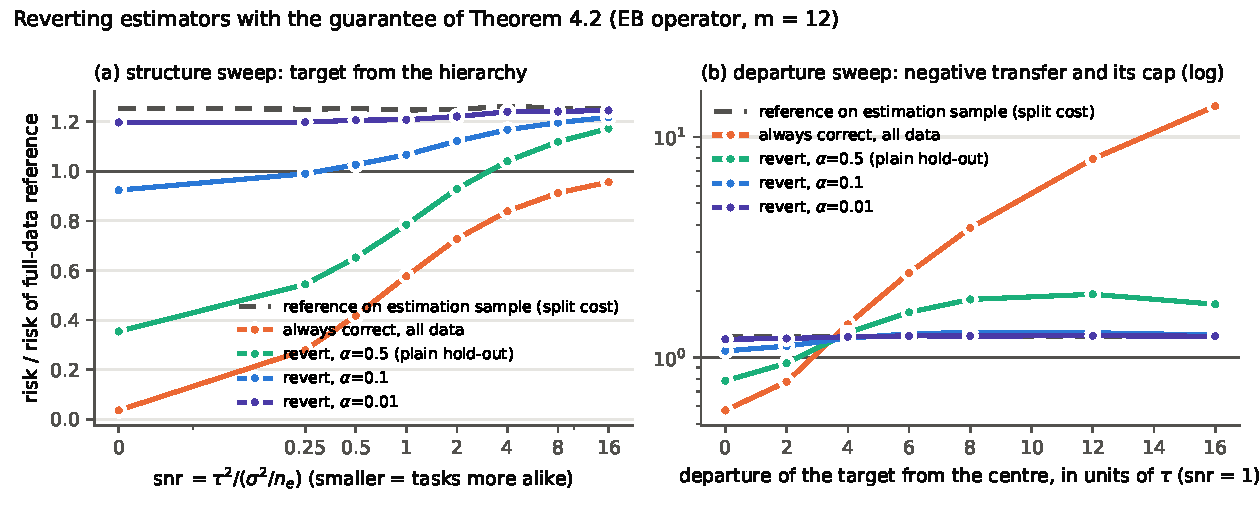
\includegraphics[width=0.68\linewidth]{../figures/sweeps.pdf}
\caption{Reverting estimators with the guarantee, EB operator, risks relative to the full-data reference. (a)~Structure sweep (Table~\ref{tab:structure}): the reverting estimators start from the split cost (dashed) and recover part of the available gain. (b)~Departure sweep (Table~\ref{tab:departure}), log scale: always correcting is harmful from $\kappa=4$ on; at $\alpha\le0.1$ the reverting estimators stay within \DepRevLowMin--\DepRevLowMax{} times the full-data reference, and plain hold-out ($\alpha=0.5$) reaches \DepRevHalfMax{} at $\kappa=\DepRevHalfMaxAt$. The bound of Theorem~\ref{thm:safe}(ii) grows with $\E\norm{C-R}$, linearly in $\kappa$ for the shrinkage operator; what is proved for every $\kappa$ is the cap of Corollary~\ref{cor:cap}, which allows up to \UniformCapTenRatioRn{} times the full-data reference at $\alpha=0.1$ and \UniformCapHalfRatioRn{} at $\alpha=0.5$. The variants without guarantee are in the last two columns of the tables.}
\label{fig:sweeps}
\end{figure}

\begin{figure}[t]
\centering
\begin{minipage}[c]{0.53\linewidth}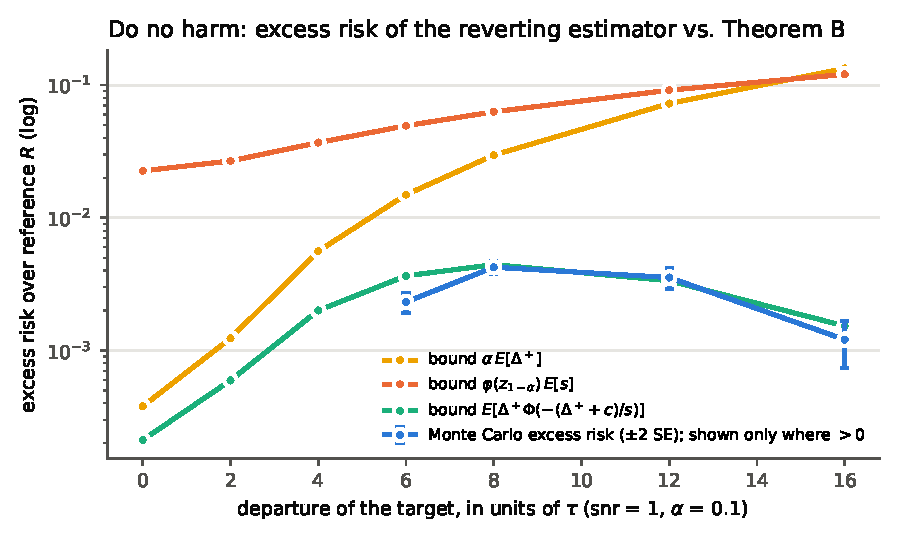
\includegraphics[width=\linewidth]{../figures/excess_vs_bounds.pdf}\end{minipage}\hfill
\begin{minipage}[c]{0.44\linewidth}
\caption{Excess risk over $R$ on the departure sweep ($\alpha=0.1$) against the bounds of Theorem~\ref{thm:safe}, the closed form $\varphi(z)\E[s]$ and the cap of Corollary~\ref{cor:cap} (dashed). The identity bound $\E[\Delta^+\pi]$ is nearly attained where the excess is positive; at $\kappa=8$ the $\kappa$-bound is \DEightRevTenBoundKappa{} against an excess of \DEightRevTenExcess; at $\kappa=16$ the cap (\UniformCapTen) is below the $\kappa$-bound (\DSixteenRevTenBoundKappa).}
\label{fig:excess}
\end{minipage}
\end{figure}

\paragraph{Results: safety (S).}
Across all \CnConfigs{} (configuration, operator, $\alpha$) combinations the bounds of Theorem~\ref{thm:safe}(i)--(ii), in the $\kappa$-form and in the closed form, hold with the two-standard-error allowance: \SafeAll; the harmful-event frequency bound holds: \SafeHarmAll; the cap of Corollary~\ref{cor:cap} holds: \SafeUniformAll{} (largest ratio of excess to cap \MaxExcessOverUniform; at $m=\Cm$ and $\alpha=0.1$ the cap is \UniformCapTen, \UniformCapTenOverRe{} times the risk of $R$ and \CapPhiOverCapTen{} times smaller than its closed form \CapPhiTen; the $\kappa$-bound exceeds it by up to \MaxBoundKappaOverUniform{} times on the grid). In this design the worst case over operators at $\alpha=0.1$ lies between \WorstLowerTen{} and \WorstUpperTen{} (Proposition~\ref{prop:sharp}(b)). Where $\Delta>0$ almost surely, the comparison with $\E[\Delta^+\pi]$ is a check of identity~(i) between two Monte Carlo estimates of the same quantity, not of a bound. The largest ratio of the Monte Carlo excess to the $\kappa$-bound is \MaxExcessOverKappa, to its closed form $\varphi(z)\E[s]$ \MaxExcessOverPhi, and to the regret bound of Theorem~\ref{thm:safe}(iv) it is \MaxRegretOverBound. The identity of Theorem~\ref{thm:safe}(i) was checked replicate by replicate: paired $z$-test where acceptance is frequent (\NIdentityCLT{} combinations, largest $|z|$ \MaxIdentityZ), Poisson 99\% interval for the acceptance count where it is rare (\NIdentityPoisson{} combinations, \NIdentityFail{} failure: \RecheckConfig, \RecheckMainCount{} acceptances against \RecheckMainExpected{} expected, not reproduced with \RecheckSeeds{} fresh seeds, \RecheckCount{} against \RecheckExpected, $z=\RecheckZ$); a conditional check with a fixed $(R,C,\theta)$ agrees with $\Phi(-(\Delta+zs)/s)$ at every $\alpha$ (largest $|z|$ \CondCheckMaxZ). The frequency of harmful events (the correction used and harmful) of the EB operator never exceeds \HarmMaxHalf{} at $\alpha=0.5$, \HarmMaxTen{} at $\alpha=0.1$ and \HarmMaxOne{} at $\alpha=0.01$, against up to \DSixteenAlwaysEHarm{} for always correcting on the split sample; the frequency of using $C$ given that it is harmful never exceeds $\alpha$ (at most \AccHarmMaxTen{} for $\alpha=0.1$). Reversion also caps the two bad operators: full pooling has unreverted risk \SSixteenPoolAlways{} at $\snr=16$ against \SSixteenPoolRevTen{} after reversion (the per-configuration tables for all operators, with every bound, are in \path{results/tables.md}, T1, T2 and T4).

\paragraph{Results: usefulness (U).}
Always correcting with all the data is useful at $\snr\in\{$\UsefulAlways$\}$ and, in the hierarchy, never harmful in the criterion's sense; its relative gain over $\bar X_n$ is \SOneAlwaysGain{} at $\snr=1$. The reverting estimator \emph{with} the guarantee is useful at $\snr\in\{$\UsefulRevHalf$\}$ for $\alpha=0.5$, $\{\UsefulRevTwenty\}$ for $\alpha=0.2$, $\{\UsefulRevTen\}$ for $\alpha=0.1$, and nowhere for $\alpha\le0.05$: at $\snr=1$ its gain over $\bar X_n$ is \SOneRevHalfGain{} ($\alpha=0.5$), \SOneRevTenGain{} ($\alpha=0.1$) and \SOneRevOneGain{} ($\alpha=0.01$), while its gain over the reference on the same estimation sample is \SOneRevHalfGainE, \SOneRevTenGainE{} and \SOneRevOneGainE. The difference is the split cost of Corollary~\ref{cor:split} (\SplitCost{} of the full-data risk, \SplitCostR{} of the risk of $R$), which the guarantee does not cover, plus the gain forfeited by the test (Remark~\ref{rem:power}): at $\snr=1$ and $\alpha=0.1$ the correction is used in \SOneRevTenAcc{} of the replicates although it helps in \SOneAlwaysEHelp{} of them. The held-out-size sweep (\path{results/tables.md}, T3; $\tau^2$ fixed, so that the estimators that do not use the split stay flat in $m$) shows the trade-off: with $m=3$ (a \MThreeSplit{} split) the gain of the guaranteed estimator over $\bar X_n$ is \MThreeZeroRevGain{} at $\kappa=0$ and \MThreeEightRevGain{} at $\kappa=8$, with excess \MThreeEightExcess{} over $R$ ($\kappa$-bound \MThreeEightBoundKappa); with $m=24$ it is \MTwentyFourZeroRevGain{} and \MTwentyFourEightRevGain. The two variants without guarantee are useful over a wider range: refit at $\snr\in\{$\UsefulRefitTen$\}$ ($\alpha=0.1$) and SURE reversion at $\snr\in\{$\UsefulSure$\}$, the latter within a few points of always correcting in the hierarchy. \NBorderline{} of the marks in Table~\ref{tab:structure} are borderline (lower end of the interval within \BorderPts{} points of the threshold): \BorderlineList; in particular ``refit useful up to $\snr=1$'' should not be read as robust (the reduced run, \texttt{--fast} with $4\,000$ replicates, keeps every other mark and drops that one).

\paragraph{Results: negative transfer.}
On the departure sweep always correcting with all the data becomes harmful (upper end of the 95\% interval of the gain below zero) at $\kappa\in\{$\HarmfulAlwaysDep$\}$ and reaches \DSixteenAlwaysRatio{} times the full-data reference risk at $\kappa=16$. The guaranteed reverting estimator at $\alpha=0.1$ stays between \DZeroRevTenRatio{} and \DEightRevTenRatio{} times the full-data reference over the whole sweep; its excess over $R$ is \DEightRevTenExcess{} at $\kappa=8$ against the bounds \DEightRevTenBoundTight{} (identity), \DEightRevTenBoundKappa{} ($\kappa$) and \DEightRevTenBoundAlpha{} ($\alpha$), and \DSixteenRevTenExcess{} at $\kappa=16$ against \DSixteenRevTenBoundKappa{} ($\kappa$) and the cap \UniformCapTen. The unguaranteed variants are also capped in this design (SURE reversion is harmful only at $\kappa\in\{$\HarmfulSureDep$\}$, by at most \DFourSureRatio{} times the reference), but nothing proved here says they must be.

\paragraph{Results: transported refit and cross-fitting.}
In all \RfDesignN{} (configuration, operator, $\alpha$) combinations the excess of the transported refit over $\bar X_n$ stays below the bounds of Theorem~\ref{thm:refit}(ii) and (iii) (largest ratios \RfDesignMaxB{} and \RfDesignMaxCap; \RfDesignMaxBc{} and \RfDesignMaxCapc{} to the closed forms); identity~(i), checked replicate by replicate, gives $|z|\le\RfIdMaxZ$ in \RfIdNz{} combinations and \RfIdFail{} Poisson failure in \RfIdNPois{} rare-acceptance ones. On an adversarial grid of \RfAdvN{} pairs $(\theta,C)$ all bounds hold within two standard errors (largest ratio \RfAdvMaxCap{} to the exact cap, at $\alpha=0.01$), a family built from the maximiser of $M_\eta$ reaches \RfAdvWorstMin--\RfAdvWorstMax{} times the exact cap and the reflection of (iv) \RfAdvReflMin--\RfAdvReflMax{} times its value, and identity~(i) gives $|z|\le\RfAdvIdMaxZ$ over \RfAdvIdN{} points (\RfAdvIdAbove{} above the threshold 3 fixed in advance). The cross-fitted estimator ($m\in\{\RfCfMs\}$) satisfies Corollary~\ref{cor:crossfit} in all \RfCfN{} design and \RfAcfN{} adversarial combinations, loosely (largest ratio \RfCfMaxB{} to the bound in the design).

In the design (EB operator, $\alpha=0.1$, $m=\Cm$; per-configuration values in \path{theory/check_refit_output.txt}) the transported refit does not pay the split: in the hierarchy its gain over $\bar X_n$ at $\alpha=0.1$ is \SZeroTrTenGain{} at $\snr=0$ and \SOneTrTenGain{} at $\snr=1$, and criterion~U (applied after the fact to this estimator, added in v0.4) holds at $\snr\in\{\UsefulTrHalf\}$ for $\alpha=0.5$, $\{\UsefulTrTwenty\}$ for $0.2$ and $\{\UsefulTrTen\}$ for $0.1$. It is not harmless: on the departure sweep it is harmful relative to $\bar X_n$ at $\kappa\in\{\HarmfulTrTenDep\}$ for $\alpha=0.1$, with risk at most \DepTrTenMax{} times that of $\bar X_n$ ($\kappa=\DepTrTenMaxAt$; \DepTrHalfMax{} at $\alpha=0.5$, $\kappa=\DepTrHalfMaxAt$), within the proved bounds. Cross-fitting with $K=\RfCfK$ folds gains \RfCfSZeroGain{} over $\bar X_n$ at $\snr=0$, and its excess on the departure sweep never exceeds \RfCfDepMax. The simulation's refit (operator re-applied) also stays below the bounds of Theorem~\ref{thm:refit} (largest ratios \RfSimMaxB{} and \RfSimMaxCap), but this is empirical only.



\paragraph{Verdict under the predefined criterion.}
Safety holds everywhere, as it must. Useful transfer with the guaranteed construction occurs only when the tasks are close ($\snr\le\UsefulRevMaxHalf$ with plain hold-out, only $\snr=\UsefulRevMaxTen$ at $\alpha=0.1$, never at $\alpha\le0.05$), because elsewhere the split costs more than the transfer gains. The transported refit of Section~\ref{sec:refit} removes the split cost for each given correction and is useful over a wider range with plain hold-out, but its worst case retains at least the fraction $4\alpha$ of the split cost (Table~\ref{tab:worstrefit}); its bound and the cross-fitted one are proved here but not yet independently refereed. The other constructions useful over a wide range are classical (empirical Bayes shrinkage with SURE selection; cross-validated selection and refit with the operator re-applied), with no finite-sample ``do no harm'' bound proved here.

\section{Claims and their status}\label{sec:claims}

\begin{table}[htbp]
\centering\footnotesize
\begin{tabular}{L{0.69\linewidth}L{0.25\linewidth}}
\toprule
claim & status\\
\midrule
No estimator using source data whose law is free of $\theta$ beats the minimax risk $d\sigma_e^2$ (a); a fixed additive correction is worse by exactly $\E\norm b^2$ at every $\theta$ (b); for $d\le2$ any rule that ever corrects is worse than $R$ somewhere (c); for $d\ge3$ pointwise but not worst-case improvement exists (d) (Thm.~\ref{thm:nfl}) & (a) classical, proof included; (b) proved here; (c) literature${}+{}$proved here; (d) literature\\
Bayes and frequentist risk of affine shrinkage; available gain $1/(1+\snr)$ (Rem.~\ref{rem:enter}) & classical\\
Held-out loss difference conditionally unbiased, Gaussian with sd $2\sigma\norm{C-R}/\sqrt m$ (Lem.~\ref{lem:unbiased}); excess-risk identity $\E[\Delta\pi]$ (Thm.~\ref{thm:safe}(i)) & proved here; identity checked in \CnConfigs{} combinations\\
Harm $\le\min\{\alpha\E\Delta^+,\kappa(\alpha)2\sigma\E\norm{C-R}/\sqrt m\}$, closed form $\varphi(z)\ge\kappa(\alpha)$; $\Prob(C\text{ used},\Delta>0)\le\alpha\Prob(\Delta>0)$; Hoeffding version; near-oracle selection within $(z+\varphi(0))2\sigma\E\norm{C-R}/\sqrt m$ (Thm.~\ref{thm:safe}(ii)--(iv)) & proved here; every bound holds everywhere (S)\\
Cap uniform in $\theta$ with constants $(\kappa,\kappa_2)$, for any measurable $C$ (Cor.~\ref{cor:cap}) & proved here; holds everywhere\\
Total cost relative to the full-data reference $=$ split cost ($m/n_e$ of its risk) $+$ controlled term (Cor.~\ref{cor:split}) & proved here\\
Within one-sided checks at a fixed level $\alpha$: $\kappa(\alpha)$ is the best constant; for a fixed estimation sample the worst-case harm over operators is of exact order $m^{-1/2}$ (Prop.~\ref{prop:sharp}) & proved here; constants numerical; (b) checked by Monte Carlo\\
Reverting estimator $=$ penalised hold-out selection between two candidates; hence no differentiation is to be expected from the safety mechanism itself (Prop.~\ref{prop:select}, Sec.~\ref{sec:related}) & proved here\\
Differentiation through the operator family & not explored (three affine instances)\\
Useful transfer (criterion U) only at $\snr\in\{$\UsefulRevHalf$\}$ ($\alpha=0.5$), $\{$\UsefulRevTwenty$\}$ ($0.2$), $\{$\UsefulRevTen$\}$ ($0.1$), never for $\alpha\le0.05$, in this design & verified, design-specific; \NBorderline{} marks borderline\\
Transported refit: exact identity; bound proportional to $\norm{C-R}$; cap uniform in $\theta$ and $C$, never below $4\alpha$ times the split cost (Thm.~\ref{thm:refit}); cross-fitted version (Cor.~\ref{cor:crossfit}) & proved here, \emph{not yet independently refereed}; constants numerical; all bounds hold (MC)\\
Worst case of the transported refit below that of the split estimator for $\alpha\le0.05$, above it for $\alpha\ge0.2$ (Table~\ref{tab:worstrefit}) & numerical, design-specific\\
``$C$ if the check passes, else $\bar X_n$'' keeps \RfVOneMin--\RfVOneMax{} of the split cost (Rem.~\ref{rem:refitcost}(c)) & derived here; quadrature\\
Refit as simulated (operator re-applied to $\bar X_n$) and SURE reversion useful over a wider range and capped in this design & empirical; no guarantee (not covered by Thm.~\ref{thm:refit})\\
General accuracy improvement, transfer guarantee, statements about real populations & not claimed\\
\bottomrule
\end{tabular}
\caption{Claims and their status. ``Verified'' and ``holds'' mean reproduced by the script of Appendix~\ref{app:repro} with the fixed seed; neither is a proof.}
\label{tab:claims}
\end{table}

\paragraph{Limitations.}
The model is Gaussian location with known variance; the $\kappa$-bound and the cap use Gaussian held-out observations, the Hoeffding version needs bounded ones, and the $t$-test variant is only remarked on. The reference is the sample mean; for a biased reference (a shared instrument bias, say) the held-out sample of the target carries the same bias and the check cannot see the correction, so that setting needs unbiased calibration data and is not covered. The simulation has one design ($d=\Cd$, $n=\Cn$, $S=\CS$) and one structural family; the ``useful'' region depends on the split fraction and on the dimension through the ratio of the $\kappa$-bound to the reference risk, of order $\sqrt{n_e/m}/\sqrt d$ for the shrinkage operator, and would move in another design. The unguaranteed variants are reported, not analysed. Theorem~\ref{thm:refit} and Corollary~\ref{cor:crossfit} were derived in a separate pass, re-derived by the integrating pass and checked by Monte Carlo, but have not yet been through an independent referee; for the transported refit no analogue of the $\alpha$-form or of the harmful-event bound is proved. Nothing is said about real data.

\paragraph{Next steps for the research line.}
(a)~\emph{Partially closed in v0.4} (Section~\ref{sec:refit}): the transported refit and its cross-fitted version have finite-sample bounds; open are a bound for the refit as simulated (operator re-applied), an $\alpha$-form and a harmful-event bound for the transported refit, a cross-fitting bound that exploits the averaging instead of Jensen's inequality, and an independent referee of Theorem~\ref{thm:refit}. (b)~A selection bound for SURE reversion with the affine operator, whose selection region is a ball around $\hat\mu$ and whose risk is not given by SURE because of the discontinuity on the sphere. (c)~If the original operator definitions of OMR001 are recovered, place each in Table~\ref{tab:constructs} and compute $\E\norm{C-R}$ for it; by Theorem~\ref{thm:safe} that is all the safety analysis needs, and such a family is the only remaining source of differentiation. (d)~Decide whether the line should be closed with this note or continued only along (a)--(b).

\appendix
\section{Reproducibility}\label{app:repro}
{\sloppy The folder contains \path{experiments/safe_reversion.py} (all sweeps, constants, identity re-checks, tables and figures; \texttt{--fast} runs a reduced version) and \path{experiments/make_numbers.py}, which converts \path{results/results.json} into the macros and table bodies of this document, so that every number in the text is generated and none is typed. The full run used seed \MetaSeed{} (re-checks: \MetaSeed{}${}+1$ and \MetaSeed{}${}+1000+i$), Python \MetaPython, NumPy \MetaNumpy~\citep{harris2020}, SciPy \MetaScipy~\citep{virtanen2020} and Matplotlib \MetaMpl~\citep{hunter2007}, and took \MetaSeconds{}~s of wall-clock time (\MetaCPUSeconds{}~s of CPU) on a shared four-core machine. \path{experiments/check_uniform_cap.py} (seconds; no number in the text comes from it) checks Corollary~\ref{cor:cap} on a grid and Proposition~\ref{prop:sharp}(b) by Monte Carlo. Since v0.4, \path{theory/check_refit.py} (\RfReps{} replicates per point, seeds \MetaSeed, ${}+7$, ${}+11$, ${}+13$; \RfCPU~s of CPU) checks Section~\ref{sec:refit} and writes \path{results/refit_check.json}, whose SHA-256 (prefix \texttt{\RfSHA}) is recorded in \path{results/refit_check.json.sha256} and verified by \path{make_numbers.py}.\par}

\paragraph{Procedure.} Criterion U was fixed in writing before the runs (script docstring and \path{results.json}). The two-standard-error tolerance of S and the thresholds of the identity check ($|z|\le3$, Poisson 99\%) were chosen before the final run but not recorded beforehand. The Poisson comparison replaced a paired $z$-test after a first run showed that the normal approximation fails where acceptance is rare. After the first internal review the held-out-size sweep was re-run with $\tau^2$ fixed and the borderline mark was introduced; after the second, checks against the $\kappa$-form of Theorem~\ref{thm:safe}(ii) and against the cap with $(\kappa,\kappa_2)$ were added, and maxima quoted as ``never exceeds'' are rounded up; no simulated number changed. No other change to the protocol or the criteria was made after seeing results. Proposition~\ref{prop:sharp}(b) and the constants $\kappa,\kappa_2$ in Theorem~\ref{thm:safe}(ii) and Corollary~\ref{cor:cap} are due to the second internal review. Risks are Monte Carlo means with standard errors from the replicate standard deviation; relative gains use paired differences and treat the denominator as fixed (its relative standard error is below $1\%$); $\kappa(\alpha)$ and $\kappa_2(\alpha)$ are computed by \path{scipy.optimize.minimize_scalar} on $[0,20]$, which contains both maximisers (at most \UStarMax{} and \UTwoStarMax), with tolerance $10^{-10}$. The draws per replicate are listed in the README; the constants in Table~\ref{tab:constants}.

\begin{table}[htbp]
\centering\footnotesize
\begin{tabular}{rrrrrrrrr}
\toprule
$\alpha$ & $z_{1-\alpha}$ & $\varphi(z_{1-\alpha})$ & $\kappa(\alpha)$ & $u^\ast$ & $\kappa/\varphi(z_{1-\alpha})$ & $\kappa_2(\alpha)$ & $\kappa_2/\varphi(1)$ & $z_{1-\alpha}+\varphi(0)$\\
\midrule
0.5 & 0.000 & 0.3989 & 0.1700 & 0.752 & 0.426 & 0.1657 & 0.685 & 0.399 \\
0.2 & 0.842 & 0.2800 & 0.0451 & 0.543 & 0.161 & 0.0331 & 0.137 & 1.241 \\
0.1 & 1.282 & 0.1755 & 0.0188 & 0.465 & 0.107 & 0.0120 & 0.049 & 1.680 \\
0.05 & 1.645 & 0.1031 & 0.0082 & 0.413 & 0.079 & 0.0047 & 0.019 & 2.044 \\
0.01 & 2.326 & 0.0267 & 0.0013 & 0.337 & 0.049 & 0.0006 & 0.003 & 2.725
\\
\bottomrule
\end{tabular}
\caption{Constants of Theorem~\ref{thm:safe}, Corollary~\ref{cor:cap} and Proposition~\ref{prop:sharp}: $\kappa(\alpha)=\sup_{u\ge0}u\Phi(-(z_{1-\alpha}+u))$, attained at $u^\ast$, and $\kappa_2(\alpha)=\sup_{u\ge0}u^2\Phi(-(z_{1-\alpha}+u))$; $\varphi(1)=\PhiOne$.}
\label{tab:constants}
\end{table}

\section{Proofs for Section~\ref{sec:refit}}\label{app:proofs}
{\small

\begin{proof}[Proof of Theorem~\ref{thm:refit}]
Write $h=\Ybar-\theta$, so that $\bar X_n-\theta=(1-\eta)e+\eta h$ and, because $J^2=J$ and $\Delta=\norm w^2+2\ip{w,e}$,
\[
\ell(\hat\theta_{\rm rf})-\ell(\bar X_n)=J\big(\norm w^2+2\ip{w,\bar X_n-\theta}\big)=J\big((1-\eta)\Delta+\eta\norm w^2+2\eta\ip{w,h}\big).
\]
This difference is at least $-\ell(\bar X_n)$, so all expectations below are well defined; (iii) shows that they are finite.
(i) By Lemma~\ref{lem:unbiased}, given $(\mathcal F,\theta)$ we have $\ip{w,h}=(s/2)Z$ with $Z\sim N(0,1)$ and $\Dh=\Delta-sZ$, so $J=\mathbf 1\{Z\ge z+u\}$: the check depends on the held-out sample only through $Z$. Hence $\E[J\mid\mathcal F,\theta]=\pi$ and, since $\int_\tau^\infty x\varphi(x)\,\dd x=\varphi(\tau)$, $\E[J\ip{w,h}\mid\mathcal F,\theta]=(s/2)\varphi(z+u)$. Take expectations. The second form uses $(1-\eta)\Delta+\eta\norm w^2=\Delta-2\eta\ip{w,e}$. If $s=0$, then $w=0$ and both sides vanish.
(ii) Since $\norm w^2-\Delta=-2\ip{w,e}\le2\norm w\norm e=s\xi$, we have $(1-\eta)\Delta+\eta\norm w^2\le s(u+\eta\xi)$, so the conditional excess is at most $s\,g(u)$ with $g(u)=(u+x)\Phi(-(z+u))+\eta\varphi(z+u)$ and $x=\eta\xi$; this gives the first inequality. The second follows from $\Psi_\eta(\alpha;x)\le\Psi_\eta(\alpha;0)+x$ and $s\xi=2\norm w\norm e$. For the closed form: if $u\ge0$, then $g(u)\le\kappa(\alpha)+\eta\varphi(z)+x\alpha$ (because $z\ge0$, $\varphi$ decreases on $[0,\infty)$ and $\Phi(-(z+u))\le\alpha$); if $-x\le u<0$, then $g(u)\le\eta\varphi(0)+x\Phi(x-z)$; if $u<-x$, the first term of $g$ is negative and $g(u)\le\eta\varphi(0)$. In all three cases $g(u)\le\bar\kappa_\eta+x\Phi(x-z)$, because $\alpha\le\Phi(x-z)$.
(iii) Put $\norm w=\sigma\omega/\sqrt m$ and $\Delta=\sigma^2\delta/m$. Then $s=2\sigma^2\omega/m$, $u=\delta/(2\omega)$, the conditional excess in (i) equals $(\sigma^2/m)f_\eta(\omega,\delta)$, and $|\Delta-\norm w^2|=2|\ip{w,e}|\le2\norm w\norm e$ reads $|\delta-\omega^2|\le2\xi\omega$. Since $\xi$ is a function of $e\sim N(0,\sigma^2I_d/n_e)$, whose law does not depend on $\theta$, this proves the first claim. For the closed form, $f_\eta\le2\omega\,g(u)$ with $x=\eta\xi$, as in (ii). If $\omega\le2\xi$, then $f_\eta\le4\xi\,g(u)^+\le4\xi(\bar\kappa_\eta+\eta\xi\Phi(\eta\xi-z))$. If $\omega>2\xi$, then $u\ge\omega/2-\xi>0$, so $2\omega\le4\xi+4u$ and $g(u)\ge0$; hence $f_\eta\le4\xi g(u)+4u\,g(u)\le4\xi(\bar\kappa_\eta+\eta\xi\alpha)+4\big(\kappa_2+\eta\xi\kappa+\eta\kappa_\varphi\big)$, using $u^2\Phi(-(z+u))\le\kappa_2$, $u\Phi(-(z+u))\le\kappa$ and $u\varphi(z+u)\le\kappa_\varphi$, with $\kappa_\varphi\le\sup_{t\ge0}t\varphi(t)=\varphi(1)$ since $z\ge0$. Both case bounds are at most the stated bound on $M_\eta$. Finally, with $R=\bar X_e$, $\xi\sim\sqrt{m/n_e}\,\norm Z$, so $\E\xi=c_d\sqrt{m/n_e}$, $\E\xi^2=dm/n_e$ and $\E\xi^3=\mu_{3,d}(m/n_e)^{3/2}$; also $\Phi(\eta\xi-z)\le\alpha+\eta\xi\varphi(0)$. Multiply by $\sigma^2/m$; the term $(\sigma^2/m)\,4\eta\alpha\,dm/n_e$ equals $4\alpha\,d\sigma^2m/(nn_e)$.
(iv) Parametrise $\delta=\omega^2+2\xi\omega c$ with $c\in[-1,1]$. Then $f_\eta=(\omega^2+2(1-\eta)\xi\omega c)\Phi(-(z+\omega/2+\xi c))+2\eta\omega\varphi(z+\omega/2+\xi c)$ is jointly continuous in $(\xi,\omega,c)$, extends continuously by $0$ to $\omega=0$, and tends to $0$ as $\omega\to\infty$ uniformly for $\xi$ in compacts; so $M_\eta(\alpha;\cdot)\ge0$ is continuous. Fix $\theta=\theta_0$ and $\varepsilon>0$. Choose $\Xi$ with $(\sigma^2/m)\E[M_\eta(\alpha;\xi)\mathbf 1\{\xi>\Xi\}]<\varepsilon/2$ (possible by the closed form of (iii)), put $w=0$ where $\xi>\Xi$, and on a fine enough finite partition of $[0,\Xi]$ choose $(\omega,c)$ constant on each cell so that $f_\eta\ge M_\eta-\varepsilon m/(2\sigma^2)$ on it (uniform continuity on a compact). For $d\ge2$, the vector $w=(\sigma/\sqrt m)\,\omega\,(c\,\hat e+\sqrt{1-c^2}\,\hat e_\perp)$, with $\hat e=e/\norm e$ and $\hat e_\perp$ a measurable unit vector orthogonal to $e$, realises $(\omega,\delta)$, and $C=R+w$ is a measurable function of $R$, hence $\mathcal F$-measurable. For the explicit pair, $C=2\theta_0-R$ gives $w=-2e$, $\Delta=0$, $\pi=\alpha$, $(1-\eta)\Delta+\eta\norm w^2=4\eta\norm e^2$ and $s=4\sigma\norm e/\sqrt m$; apply (i) with $\E\norm e^2=d\sigma^2/n_e$ and $\E\norm e=\sigma c_d/\sqrt{n_e}$. The second term of the result is positive, so the supremum over $C$ is at least $4\alpha$ times the split cost.
\end{proof}

\begin{proof}[Proof of Corollary~\ref{cor:crossfit}]
Each observation lies outside exactly $K-1$ folds, so $\frac1K\sum_kR_k=\bar X_n$. By convexity of the squared loss, $\ell(\hat\theta_{\rm cf})\le\frac1K\sum_k\ell(\bar X_n+J_k(C_k-R_k))$. The $k$-th term is the transported refit of Theorem~\ref{thm:refit} with estimation sample outside $I_k$, held-out sample $I_k$, $\eta=m/n=1/K$ and the same law of $\xi$.
\end{proof}

\paragraph{The route of Remark~\ref{rem:refitcost}(c).} For $\tilde\theta=JC+(1-J)\bar X_n$, $\ell(\tilde\theta)-\ell(\bar X_n)=J\big(\Delta+\norm e^2-\norm{\bar X_n-\theta}^2\big)$. Take $\theta=\theta_0$ and $C=R-t\,e$: then $|\Delta|\le(2t+t^2)\norm e^2\to0$ in $L^1$, $u\to-\xi$ and, with $Z=-\sqrt m\ip{\hat e,h}/\sigma\sim N(0,1)$ given $e$, $J\to\mathbf 1\{Z\ge z-\xi\}$ almost surely. Writing $\norm h^2=(\sigma^2/m)(Z^2+W)$ with $W\sim\chi^2_{d-1}$ independent of $Z$, using $\E[Z\mathbf 1\{Z\ge\tau\}]=\varphi(\tau)$ and $\E[Z^2\mathbf 1\{Z\ge\tau\}]=\Phi(-\tau)+\tau\varphi(\tau)$, and dominated convergence, the excess tends to
\[
\frac{\sigma^2}{m}\,\E\Big[\Phi(\xi-z)\big((2\eta-\eta^2)\xi^2-\eta^2d\big)+2\eta(1-\eta)\,\xi\,\varphi(z-\xi)-\eta^2(z-\xi)\,\varphi(z-\xi)\Big],
\]
which \path{theory/check_refit.py} evaluates by quadrature over $\xi\sim\sqrt{m/n_e}\,\chi_d$ (no Monte Carlo).\par}

\bibliographystyle{plainnat}
{\footnotesize\bibliography{refs}}
\end{document}
